\chapter{Metodologias} \label{chapter:metodologia}

Neste  capítulo  são apresentadas  as  metodologias  aplicadas para  solução  do
\gls{pma} e para análise estatística dos resultados.

\section{Fixação de Variáveis nos Modelos Matemáticos} \label{sec:prep-modelos}

Um  conjunto  de  pré-processamentos  foram   aplicados  em  ambos  os  modelos,
\gls{dmfm-pma} e \gls{ab-pma}, para fixação de variáveis. Os procedimentos foram
apresentados em Ribeiro et al. \cite{tiago:2019} e adaptados para o \gls{pma}.

Dado  um nó  terminal $k$  e um  arco $(i,  j)$ é  possível estabelecer  que uma
variável $y_{ij}$ ou $f_{ij}^{k}$ pode  ser removida do modelo, preservando pelo
menos uma solução  ótima. Para verificar a necessidade de  utilizar um arco $(i,
j)$  no caminho  da raiz  $s$  até um  terminal $k$,  são computados  limitantes
inferiores para o {\delay} e {\jitter} necessários para construir tal caminho.

Seja $r_{ij}$ um recurso associado com o arco $(i, j)$ do grafo $G$. Um terminal
$k$ só pode  ser classificado como atendido  se, para um caminho $P$  que vai da
raiz  $s$  até $k$,  a  soma  dos valores  de  $r$  não excedem  uma  quantidade
$\Delta_r$. Seja  $LB_{si}$ um limitante  inferior da quantidade de  recurso $r$
necessário para ir da  raiz $s$ até o nó $i$, e  analogamente, seja $LB_{jk}$ um
limitante inferior  da quantidade de recurso  $r$ necessário para ir  de $j$ até
$k$. Logo, se

\begin{equation}
LB_{si} + r_{ij} + LB_{jk} > \Delta_r, \label{eq:base-prep}
\end{equation}

é possível afirmar que, com a utilização do arco $(i, j)$ no caminho da raiz $s$
até  o  terminal  $k$, o  terminal  $k$  não  será  atendido. Logo,  a  variável
$f_{ij}^{k}$ pode  ser fixada em zero  ou removida do modelo.  Para o \gls{pma},
existem dois recursos a serem considerados: {\delay} e {\jitter}. Ribeiro et al.
\cite{tiago:2019}  desenvolveram  três  diferentes   variações  de  cálculo  dos
limitantes  da  Equação  \eqref{eq:base-prep}.  Este  trabalho  aplica  os  dois
procedimentos mais eficientes para eliminação de variáveis nas formulações, dado
que o terceiro procedimento é dominado pelos demais.

Considere uma  instância do  \gls{pma} definida  por um grafo  $G$ e  as funções
$\lambda$ e  $\xi$ que  representam, respectivamente, os  valores de  {\delay} e
{\jitter} de cada arco. As seguintes notações e definições são utilizadas:

\begin{itemize}
 \item $G_{\lambda}$: grafo  direcionado $G$ com os custos dos  arcos dados pela
função $\lambda$ e os recursos dados pela função $\xi$;
 \item  $G_{\xi}$: grafo  direcionado $G$  com os  custos dos  arcos dados  pela
função $\xi$ e os recursos dados pela função $\lambda$;
 \item $G^T_r$: o transposto do grafo $G_r$ para $r \in \{\lambda, \xi\}$ (i.e.,
com as direções dos arcos invertidas);
 \item $SP(r, u, v)$:  o caminho mínimo, do inglês \gls{sp}, de  $u$ para $v$ no
grafo $G_r$, onde $r  \in \{\lambda, \xi\}$ e $u$ e  $v$ correspondem à qualquer
par de nós distintos em $G_r$;
 \item $SPRC(r,  u, v,  \Delta_t)$: o caminho  mínimo de $u$  para $v$  no grafo
$G_r$  restrito a  usar  até  $\Delta_t$ unidades  de  recursos  $t$, do  inglês
\gls{sprc}, onde $r \text{ e } t \in  \{\lambda, \xi\} \text{, } r \neq t$ e $u$
e $v$ correspondem à qualquer par de nós distinto em $G_r$; e
 \item $SPRC^T(r, u, v, \Delta_t)$: mesmo que acima, mas em $G^{T}_{r}$.
\end{itemize}

Os    pré-processamentos   seguem    a   mesma    nomenclatura   utilizada    em
\cite{tiago:2019}. Os procedimentos podem ser classificados em fraco, moderado e
forte,  dependendo da  quantidade de  vezes que  os caminhos  mínimos com  e sem
restrições de  recursos são computados  para obtenção dos limitantes  da equação
\eqref{eq:base-prep}.  Os   procedimentos  utilizados  neste  trabalho   são  os
seguintes:

\noindent \paragraph*{
1. Remoção  de Vértices Moderada, do  inglês \gls{mve}:} Dado um  nó $i
\in S$ e recursos $r$ e $t \in \{\lambda, \xi\}$ com $r \neq t$, se

\begin{equation}
  {SPRC}(r, s, i, \Delta_t) + {SP}(r, i, k) > \Delta_r, \ \forall k \in D,
\end{equation} então o  vértice $i$ pode ser removido do  grafo. Isso decorre da
quantidade mínima  de recurso $r$  necessária para ir  da raiz $s$  até qualquer
terminal $k$, passando pelo nó $i$, excede  o limite permitido para que $k$ seja
atendido. A  remoção pode ser  aplicada no grafo  ou fixando todas  as variáveis
$y_{ij}, y_{ji}, f_{ij}^{k}$ e $f_{ji}^k$ para todo $k \in D$, em $0$.

\begin{comment}
Perceba que,  sem a utilização desse  pré-processamento, podem existir
soluções viáveis para  o \gls{pma} nas quais $i$ é  utilizado como intermediário
no caminho para pelo  menos um terminal. Mas, a utilização  $i$ implica que todo
terminal visitado nesse  caminho não é atendido, assim, é  possível remover o nó
$i$ e todos os arcos adjacentes a  ele. Assim, o pré-processamento garante que o
caminho para  visitar os nós  opcionais removidos passe pelos  arcos artificiais
$(s, s')$ e $(s', i)$, reduzindo assim o espaço de soluções.
\end{comment}

\noindent \paragraph*{2. Remoção  de Arcos Moderada, do  inglês \gls{mae}:} Dado
um arco $(i, j) \in A$ e recursos $r$ e $t \in \{\lambda, \xi\}$ com $r \neq t$,
se

\begin{equation}
    \text{SPRC}(r, s,  i, \Delta_t) + r_{ij}  + \text{ SP }(r,  j, k) > \Delta_r, \ \forall k \in D
  \end{equation}

então o  arco $(i, j)$  pode ser removido do  grafo. Isso decorre  da quantidade
mínima de recurso $r$ para ir da  raiz $s$ até qualquer terminal $k$, utilizando
o arco $(i,  j)$, ultrapassar o limite  permitido para que $k$  seja atendido. A
remoção  pode ser  aplicada  no  grafo ou  fixando  todas  variáveis $y_{ij}$  e
$f_{ij}^k$ para todo $k \in D$, em $0$.

\begin{comment}
O funcionamento desse pré-processamento,  aplicado ao \gls{pma},
pode ser demonstrado utilizando o  mesmo princípio descrito anteriormente para o
\gls{mve}.  
\end{comment}

\noindent \paragraph*{3. Remoção  de Arcos Forte, do inglês  \gls{sae}:} Dado um
arco $(i, j) \in A$, um terminal $k \in D$ e os recursos $r$ e $t \in \{\lambda,
\xi\}$ com $r  \neq t$, considerando a Equação \eqref{eq:base-prep}.  O valor do
limitante $LB_{si}$ pode ser computado da seguinte maneira:

\begin{equation}
    LB_{si} = SPRC(r, s, i, \Delta_t - \substack{\min \\ l \in D, l \neq i} \{SP(t, i, l)\}). \label{eq:lbsi}
 \end{equation}

Esse valor  é computado  considerando que, em  um fluxo enviado  de $s$  para um
terminal $k$ utilizando  o arco $(i, j)$, a quantidade  de recurso $t$ consumido
para ir de  $i$ até $k$ é  limitado inferiormente pelo valor  de $\min\{SP(t, i,
l): l \in D, l \neq i\}$, ou seja, o caminho mínimo em função de $t$ indo de $i$
até qualquer terminal $l \neq i$. Assim, resta no máximo $\Delta_t$ subtraído do
valor desse  caminho mínimo. Consequentemente,  o tamanho do caminho  mínimo com
restrição de recurso dado por essa fórmula é um limitante inferior da quantidade
de recurso $r$ gasto para ir da raiz $s$ até o nó $i$. O valor de $LB_{jk}$ pode
ser obtido por:

\begin{equation}
    LB_{jk} = SPRC^{T}(r, k, j, \Delta_t - SPRC(t, s, j, \Delta_r)). \label{eq:lbjk}
\end{equation}

O termo $\Delta_t  - SPRC(t, s, j, \Delta_r)$ corresponde  ao limitante superior
de recurso $t$ disponível para ir de $j$ até $k$, considerando que utilizou-se o
mínimo possível desse  recurso no caminho de  $s$ até $j$. O  motivo do computar
esse  caminho com  base  no  grafo $G^T$  está  relacionado  com a  complexidade
computacional e será discutida posteriormente. Finalmente, se

\begin{multline}
  \left( SPRC(r, s, i, \Delta_t - \substack{\min \\ l \in D, l \neq i} \{SP(t, i, l)\})\right) + r_{ij}\\ +
  SPRC^{T}(r, k, j, \Delta_t - SPRC(t, s, j, \Delta_r)) > \Delta_r,
\end{multline}
então o  arco $(i, j)$ pode  ser removido do caminho  que vai da raiz  $s$ até o
terminal  $k$. Para isso, a variável $f_{ij}^k$ é fixada em zero.

Ribeiro  et al.  \cite{tiago:2019} apresentam  a complexidade  computacional dos
testes  propostos.  Toda computação  é  feita  no grafo  $G  =  (V, A)$  ou  seu
transposto. Sendo $n = |V|$, $m = |A|$ e  o número de nós terminais $d = |D|$, o
tempo de execução dos testes depende diretamente do custo computacional de gerar
os caminhos em cada caso. Sejam  $\#SP$ e $\#SPRC$ as complexidades de computar,
respectivamente,  caminhos mínimos  sem e  com restrição  de recurso  em $G$  ou
$G^T$. $\#SP$  tem complexidade $(n^2)$  com apenas um  nó raiz e  $O(n^3)$ para
computar cominho mínimos entre todos os  pares de vértices (ver, e.g., Cormen et
al.,  \cite{cormen:2009}).  Por  outro   lado,  computar  caminhos  mínimos  com
restrição de recurso é $\mathcal{NP}-$difícil.  Assim, a complexidade dos testes
é dada por  (a) MVE: $O(n \cdot \#SPRC  + n^2 \cdot \#SP)$; (b)  MAE: $O(n \cdot
\#SPRC + n^2 \cdot \#SP)$; e (c) SAE: $O(n \cdot \#SPRC + n^2 \cdot \#SP) + O((d
+ n) \cdot \#SPRC)$, de modo que o primeiro e segundo termos do último somatório
são as  complexidades associadas às Equações  \eqref{eq:lbsi} e \eqref{eq:lbjk},
respectivamente.

Note  que, com  a  utilização do  algoritmo de  Floyd-Warshall  para computar  o
caminho  mínimo  entre  todos  os  pares, os  termos  $n^2  O(\#SP)$  podem  ser
substituídos por  $O(n^3)$. Ainda,  veja que no  segundo termo  correspondente à
complexidade  do teste  SAE,  utiliza-se o  do grafo  transposto  para evitar  o
cômputo de  caminhos mínimos com restrição  de recursos entre todos  os pares de
nós em $V\backslash \{s\}$. Isso ocorre pela possibilidade de restringir somente
os terminais do conjunto de nós utilizados como raiz.

Mesmo  com  o  problema  de  caminho  mínimo  com  restrição  de  recurso  sendo
$\mathcal{NP}$-difícil,  existem algoritmos  exatos  rápidos  o suficiente  para
resolver  este  problema  na  prática \cite{irnich:2006}.  A  implementação  dos
pré-processamentos utilizam o algoritmo de configuração de rótulos disponível na
biblioteca   Boost   C++   \cite{boost:2020}.   Os  tempos   de   execução   dos
pré-processamentos para  a maioria das  instâncias geradas neste  trabalho foram
irrelevantes se  comparado com o tempo  de execução do resolvedor  de \gls{pli}.
Mais detalhes sobre os pré-processamentos são descritos na Seção \ref{sec:prep}.

\section{Relaxações Lagrangianas} \label{sec:rl-pma}

\newcommand{\mult}[2]{\ensuremath{\phi^{#1}_{#2}}}

Nesta   seção,  são   apresentadas  \gls{rl}s   obtidas  a   partir  do   modelo
\gls{dmfm-pma},  proposto na  Seção  \ref{sec:dmfm-pma}.  Os multiplicadores  de
Lagrange     estão    representados     por     $\phi$'s,     de    modo     que
\mult{\ref{eq:rel-f-y-term}}{},                 \mult{\ref{eq:mod-lim-delay}}{},
\mult{\ref{eq:mod-lim-jitter}}{}   e    \mult{\ref{eq:mod-var-delay}}{},   todas
variáveis   reais   não   negativas,   estão  associados   com   as   restrições
\eqref{eq:rel-f-y-term},  \eqref{eq:mod-lim-delay}, \eqref{eq:mod-lim-jitter}  e
\eqref{eq:mod-var-delay}, respectivamente.  Todas as  relaxações mantém,  em seu
\gls{ppl}, problemas de caminho mínimo, do inglês \gls{sp} ou caminho mínimo com
restrições de recurso, do inglês  \gls{sprc}. A nomenclatura utilizada para cada
relaxação segue o padrão RL-X, onde  ``X'' representa o subproblema mais difícil
de ser resolvido do \gls{ppl}.

\subsection{Relaxação Lagrangiana - Caminho Mínimo} \label{subsec:rl-sp}

A \gls{rl}  que resulta da  dualização das restrições  \eqref{eq:rel-f-y-term} e
\eqref{eq:mod-lim-delay}-\eqref{eq:mod-var-delay} é bastante próxima do problema
de computar  \gls{sp}s e, por isso,  é denominada RL-SP. De  fato, as restrições
\eqref{eq:fluxo-raiz}-\eqref{eq:fluxo-terminal} modelam caminhos mínimos da raiz
$s$ para os demais nós do  grafo, utilizando as variáveis $f_{ij}^{k}$ para todo
$k  \in D  \cup S$.  Considerando as  variáveis $y_{ij}$,  o problema  associado
consiste na seleção do arco $(s, s')$  juntamente com os $|V'|-2$ arcos de menor
coeficiente  computados  a  partir  dos  multiplicadores  lagrangianos.  Como  o
\gls{ppl} não contém restrições que se  apliquem às variáveis $z_k$ para todo $k
\in D$,  o problema  associado com  essas variáveis consiste  na decisão  de não
atender o  terminal $k$  ($z_k =  1$) se o  coeficiente gerado,  considerando os
multiplicadores lagrangianos,  for menor  que zero, caso  contrário, $z_k  = 0$.
Assim,     ao    dualizar     as     restrições    \eqref{eq:rel-f-y-term}     e
\eqref{eq:mod-lim-delay}-\eqref{eq:mod-var-delay}, o \gls{ppl} resultante é:

% \vspace*{-0.2cm}
\begin{align}
\text{(RL-SP)} \quad 
    % Z
    & \nonumber \displaystyle \min \sum_{k \in D}z_k (1 - \mult{\ref{eq:mod-lim-delay}}{k}M_d - \mult{\ref{eq:mod-lim-jitter}}{k}M_j - \sum_{\substack{l \in D \\ l \neq k}}(\mult{\ref{eq:mod-var-delay}}{kl}M_v^k + \mult{\ref{eq:mod-var-delay}}{lk}M_v^l)) & \\ 
    % f to terminals
    & \nonumber \displaystyle + \sum_{k \in D} \sum_{(i, j) \in A'} f_{ij}^{k} (\mult{\ref{eq:rel-f-y-term}}{ijk} + \xi_{ij} \mult{\ref{eq:mod-lim-jitter}}{k} + \lambda_{ij} (\mult{\ref{eq:mod-lim-delay}}{k} + \sum_{\substack{l \in D \\ l \neq k}} (\mult{\ref{eq:mod-var-delay}}{kl} - \mult{\ref{eq:mod-var-delay}}{lk}) ) ) & \\
    & \nonumber \displaystyle + \sum_{q \in S} \sum_{(i, j) \in A'} f_{ij}^{q}(\mult{
    \ref{eq:rel-f-y-term}}{ijk}) - \sum_{k \in D \cup S} \sum_{(i, j) \in A'} y_{ij}(\mult{\ref{eq:rel-f-y-term}}{ijk}) & \\ 
    % Constant
    & \displaystyle - \sum_{k \in D} (\mult{\ref{eq:mod-lim-delay}}{k} \Delta_d + \mult{\ref{eq:mod-lim-jitter}}{k} \Delta_j + \sum_{\substack{l \in D \\ l \neq k}}(\mult{\ref{eq:mod-var-delay}}{kl} \Delta_v)) & \label{eq:fo-rlsp} \\
\nonumber \text{s.a.:} \\ \quad
    & \nonumber \eqref{eq:fluxo-raiz}-\eqref{eq:fluxo-terminal}, \eqref{eq:num-arestas-arvore} \text{ e } \eqref{eq:force-dummy-node}  & 
\end{align}

Foram utilizadas duas abordagens para  resolução do RL-SP. A primeira estratégia
de  resolução do  \gls{ppl} utiliza  resolvedor  de \gls{pli}  para obtenção  de
soluções a  cada iteração  do método  de subgradiente.  Na segunda  abordagem, a
resolução  do  \gls{ppl} consiste  em  resolver  os subproblemas  associados  ao
conjunto de  variáveis ($f,  y$ e $z$)  utilizando algoritmos  combinatórios. Um
fato  importante, que  influencia na  complexidade de  resolução do  problema de
\gls{sp},  está  relacionado  com  a  possibilidade  de  existirem  coeficientes
negativos associados às variáveis $f_{ij}^{k}$. Consequentemente, ao computar um
\gls{sp}, a  solução retornada pode  conter ciclos  negativos, o que  implica no
valor da função  objetivo do \gls{ppl} ser igual a  $-\infty$. Para evitar essas
situações, foi  explorada a resolução  de uma  versão simplificada de  {\rlu} na
qual  descarta-se  um  subconjunto   de  multiplicadores,  mais  especificamente
\mult{\ref{eq:mod-var-delay}}{}. Desconsiderar  esses multiplicadores  da função
objetivo  impede a  existência  de  arcos, associados  às  variáveis $f$,  cujos
coeficientes sejam negativos. Assim, a  nova função objetivo, denominada RL-SP',
pode ser descrita do seguinte modo:

% O resolvedor  de \gls{pli}  é capaz  computar o \gls{ppl}  e formar  os caminhos
% independente  da existência  de  ciclos negativos,  diferente  da abordagem  com
% algoritmos  combinatórios. Assim,  para  utilizar o  algoritmo  de \gls{sp}  são
% necessárias alterações  na estrutura  da relaxação. Uma  possibilidade explorada
% consiste na resolução  de uma versão simplificada de RL-SP,  

\begin{align}
\text{(RL-SP')} \quad 
    % Z
    & \nonumber \displaystyle \min \sum_{k \in D}z_k (1 - \mult{\ref{eq:mod-lim-delay}}{k}M_d - \mult{\ref{eq:mod-lim-jitter}}{k}M_j) & \\ 
    % f to terminals
    & \nonumber \displaystyle + \sum_{k \in D} \sum_{(i, j) \in A'} f_{ij}^{k} (\mult{\ref{eq:rel-f-y-term}}{ijk} + \xi_{ij} \mult{\ref{eq:mod-lim-jitter}}{k} + \lambda_{ij} \mult{\ref{eq:mod-lim-delay}}{k}) & \\
    & \nonumber \displaystyle + \sum_{q \in S} \sum_{(i, j) \in A'} f_{ij}^{q}(\mult{
    \ref{eq:rel-f-y-term}}{ijk}) - \sum_{k \in D \cup S} \sum_{(i, j) \in A'} y_{ij}(\mult{\ref{eq:rel-f-y-term}}{ijk}) & \\ 
    % Constant
    & \displaystyle - \sum_{k \in D} (\mult{\ref{eq:mod-lim-delay}}{k} \Delta_d + \mult{\ref{eq:mod-lim-jitter}}{k} \Delta_j) & \label{eq:fo-rlsp-weaker}
\end{align}

A respeito da complexidade da versão combinatória da relaxação RL-SP', considere
$n = |V|, m = |A|$, $d =  |D|$ e $\#SP$ como a complexidade de computar caminhos
mínimos em $G'$. Ainda, considere $G^k =  (V', A{'}^{k})$ para todo $k \in D\cup
S$, como subgrafo de $G'$ induzido pelas variáveis $f_{ij}^{k}$. A diferença nos
arcos  do   conjunto  $A{'}^k$,  para  cada   $k$,  se  deve  à   utilização  do
pré-processamento SAE. Assim, o problema combinatório associado às variáveis $f$
tem complexidade $O((n-1) \cdot \#SP)$. Para  as variáveis $y$, a complexidade é
dada pela ordenação dos arcos de $A'$ com os coeficientes lagrangianos, ou seja,
$O(m \log m)$. Por fim, o  problema computacionalmente mais simples, podendo ser
resolvido  em  $O(d)$,  consiste   em  verificar  os  coeficientes  lagrangianos
associados a cada variável $z$.

\subsection{Relaxação Lagrangiana - Caminho Mínimo com Restrição de {\delay}} \label{subsec:rl-sprc-delay}

A \gls{rl} obtida a partir  da dualização das restrições \eqref{eq:rel-f-y-term}
e \eqref{eq:mod-lim-delay}-\eqref{eq:mod-var-delay} resulta no problema de obter
caminhos mínimos com  restrição de {\delay} e, por isso,  será referenciada como
RL-SPRC$_{\lambda}$.  considerando  as  variáveis  $f_{ij}^{k}$,  as  restrições
\eqref{eq:fluxo-raiz}-\eqref{eq:fluxo-terminal}    e    \eqref{eq:mod-lim-delay}
modelam  caminhos mínimos  com restrição  de {\delay}  indo de  $s$ para  os nós
terminais do  grafo, enquanto,  para os nós  opcionais, basta  computar caminhos
mínimos. O problema associado com as  variáveis $y_{ij}$ se mantém como descrito
na relaxação RL-SP. Para a variável  $z_{k}$ existe duas situações nas quais seu
valor se torna igual à um. O  primeiro caso ocorre se o coeficiente gerado pelos
multiplicadores lagrangianos  for menor que  zero, enquanto o segundo  caso está
associado com  os caminhos induzidos  pelas variáveis $f_{ij}^{k}$, ou  seja, se
para  visitar  o  terminal  $k$  o {\delay}  utilizado  por  um  caminho  excede
$\Delta_d$, então  $k$ torna-se não  atendido e  consequentemente $z_k =  1$. Ao
dualizar         as         restrições         \eqref{eq:rel-f-y-term}         e
\eqref{eq:mod-lim-jitter}-\eqref{eq:mod-var-delay}, o \gls{ppl} resultante é:

% \vspace*{-0.2cm}
%\interdisplaylinepenalty=10000
\begin{align}
(\text{RL-SPRC}_{\lambda}) \quad
    % z 
    & \nonumber \displaystyle \min \sum_{k \in D}z_k (1 - \mult{\ref{eq:mod-lim-jitter}}{k}M_j - \sum_{\substack{l \in D \\ l \neq k}}(\mult{\ref{eq:mod-var-delay}}{kl}M_v^k + \mult{\ref{eq:mod-var-delay}}{lk}M_v^l)) & \\ 
    % f to terminals
    & \nonumber \displaystyle + \sum_{k \in D} \sum_{(i, j) \in A'} f_{ij}^{k} (\mult{\ref{eq:rel-f-y-term}}{ijk} + \xi_{ij} \mult{\ref{eq:mod-lim-jitter}}{k} + \lambda_{ij} (\sum_{\substack{l \in D \\ l \neq k}} \mult{\ref{eq:mod-var-delay}}{kl} - \mult{\ref{eq:mod-var-delay}}{lk})) & \\
   & \nonumber \displaystyle + \sum_{k \in S} \sum_{(i, j) \in A'} f_{ij}^{k}(\mult{\ref{eq:rel-f-y-term}}{ijk}) - \sum_{k \in D \cup S} \sum_{(i, j) \in A'} y_{ij}(\mult{\ref{eq:rel-f-y-term}}{ijk})  & \\
   & \displaystyle - \sum_{k \in D} (\mult{\ref{eq:mod-lim-jitter}}{k} \Delta_j + \sum_{\substack{l \in D \\ l \neq k}} (\mult{\ref{eq:mod-var-delay}}{kl} \Delta_v)) & \label{eq:fo-sprc-delay} \\
\nonumber \text{s.a.} \\ \quad
    & \nonumber \eqref{eq:fluxo-raiz}-\eqref{eq:fluxo-terminal}, \eqref{eq:num-arestas-arvore}-\eqref{eq:mod-lim-delay} \text{ e } \eqref{eq:force-dummy-node} & 
\end{align}

Para resolver o problema combinatório  associado com as variáveis $f_{ij}^{k}$ é
necessário  obter  um conjunto  de  \gls{sp}s  e/ou \gls{sprc}s.  Primeiramente,
deve-se  resolver  dois   subproblemas  para  cada  terminal   $k$.  O  primeiro
considerando  $k$ como  atendido  e  o segundo  como  não  atendido. Esses  dois
subproblemas  estão sujeitos  aos valores  utilizados pelos  parâmetros $M_d$  e
$M_j$, conforme será melhor explicado na Seção \ref{subsec:rl-m-valor}.

%  As diferentes possibilidades e  seus respectivos impactos na complexidade
% da relaxação serão detalhados posteriormente.

Como   descrito  para   a  relaxação   {\rlu},  a   dualização  das   restrições
\eqref{eq:mod-var-delay}  possibilita  a  existência de  coeficientes  negativos
associados  às  variáveis  $f_{ij}^k$,  podendo  inviabilizar  a  utilização  do
algoritmo  de \gls{sp}.  Seguindo a  mesma simplificação  adotada anteriormente,
pode-se reescrever a função objetivo,  referenciando-a como {\rld}', do seguinte
modo:

\begin{align}
(\text{RL-SPRC'}_{\lambda}) \quad
    & \nonumber \displaystyle \min \sum_{k \in D}z_k (1 - \mult{\ref{eq:mod-lim-jitter}}{k}M_j) + \sum_{k \in D} \sum_{(i, j) \in A'} f_{ij}^{k} (\mult{\ref{eq:rel-f-y-term}}{ijk} + \xi_{ij} \mult{\ref{eq:mod-lim-jitter}}{k}) & \\
   & \displaystyle + \sum_{k \in S} \sum_{(i, j) \in A'} f_{ij}^{k}(\mult{\ref{eq:rel-f-y-term}}{ijk}) - \sum_{k \in D \cup S} \sum_{(i, j) \in A'} y_{ij}(\mult{\ref{eq:rel-f-y-term}}{ijk}) - \sum_{k \in D} (\mult{\ref{eq:mod-lim-jitter}}{k} \Delta_j) & \label{eq:fo-sprc-delay-weaker} 
\end{align}

\subsection{Relaxação Lagrangiana - Caminho Mínimo com Restrição de {\em jitter}} \label{subsec:rl-sprc-jitter}

Essa relaxação  segue as  mesmas propriedades  da relaxação  {\rld}, modificando
apenas o  recurso de {\delay}  para {\jitter}, por  esse motivo é  intitulada de
{\rlt}. Assim, removendo a  dualização das restrições \eqref{eq:mod-lim-delay} e
dualizando \eqref{eq:mod-lim-jitter}, temos o seguinte \gls{ppl}.

\begin{align}
(\text{RL-SPRC}_{\xi}) \quad 
  & \nonumber \displaystyle \min \sum_{k \in D}z_k (1 - \mult{\ref{eq:mod-lim-delay}}{k}M_d - \sum_{\substack{l \in D \\ l \neq k}}(\mult{\ref{eq:mod-var-delay}}{kl}M_v^k + \mult{\ref{eq:mod-var-delay}}{lk}M_v^l)) & \\ 
  % f to terminals
  & \nonumber \displaystyle + \sum_{k \in D} \sum_{(i, j) \in A'} f_{ij}^{k} (\lambda_{ij} (\mult{\ref{eq:mod-lim-delay}}{k} + \sum_{\substack{l \in d \\ l \neq k}} (\mult{\ref{eq:mod-var-delay}}{kl} - \mult{\ref{eq:mod-var-delay}}{lk}) ) ) & \\
  & \nonumber \displaystyle + \sum_{k \in S} \sum_{(i, j) \in A'} f_{ij}^{k}(\mult{\ref{eq:rel-f-y-term}}{ijk}) - \sum_{k \in D \cup S} \sum_{(i, j) \in A'} y_{ij}(\mult{\ref{eq:rel-f-y-term}}{ijk}) & \\
  & \displaystyle - \sum_{k \in D} (\mult{\ref{eq:mod-lim-delay}}{k} \Delta_d + \sum_{\substack{l \in D \\ l \neq k}}(\mult{\ref{eq:mod-var-delay}}{kl} \Delta_v)) & \label{eq:fo-sprc-jitter} \\
\nonumber \text{s.a.} \\ \quad
    & \nonumber \eqref{eq:fluxo-raiz}-\eqref{eq:fluxo-terminal}, \eqref{eq:num-arestas-arvore}, \eqref{eq:mod-lim-jitter} \text{ e } \eqref{eq:force-dummy-node} & 
\end{align}

E, por  motivos análogos aos  apresentados anteriormente, a função  objetivo foi
simplificada da seguinte forma.

\begin{align}
(\text{RL-SPRC'}_{\xi}) \quad 
  & \nonumber \displaystyle \min \sum_{k \in D}z_k (1 - \mult{\ref{eq:mod-lim-delay}}{k}M_d) + \sum_{k \in D} \sum_{(i, j) \in A'} f_{ij}^{k} (\lambda_{ij} \mult{\ref{eq:mod-lim-delay}}{k}) & \\
  & \displaystyle + \sum_{k \in S} \sum_{(i, j) \in A'} f_{ij}^{k}(\mult{\ref{eq:rel-f-y-term}}{ijk}) - \sum_{k \in D \cup S} \sum_{(i, j) \in A'} y_{ij}(\mult{\ref{eq:rel-f-y-term}}{ijk}) - \sum_{k \in D} (\mult{\ref{eq:mod-lim-delay}}{k} \Delta_d) & \label{eq:fo-sprc-jitter-weaker}
\end{align} 

\subsection{Relaxação Lagrangiana - Caminho Mínimo com Restrição de Múltiplos Recursos} \label{subsec:rl-cshp2}

A  \gls{rl}  obtida pela  dualização  das  restrições \eqref{eq:rel-f-y-term}  e
\eqref{eq:mod-var-delay} resulta  no problema  de computar caminhos  mínimos com
restrições de recursos, nesse caso {\delay}  e {\jitter}, e por esse motivo será
referenciada como  {\rlq}. De fato,  considerando as variáveis  $f_{ij}^{k}$, as
restrições           \eqref{eq:fluxo-raiz}-\eqref{eq:fluxo-terminal}           e
\eqref{eq:mod-lim-delay}-\eqref{eq:mod-lim-jitter} modelam \gls{sprc}s restritos
em {\delay}  e {\jitter} da  raiz $s$  até cada um  dos nós terminais  do grafo.
Enquanto, para  os nós opcionais,  basta computar  caminhos mínimos a  partir de
$s$.  Em relação  às variáveis  $y$ e  $z$, os  problemas combinatórios  a serem
resolvidos  são os  mesmos já  descritos  anteriormente. Assim,  ao dualizar  as
restrições  \eqref{eq:rel-f-y-term}  e   \eqref{eq:mod-var-delay},  o  \gls{ppl}
resultante e:

\begin{align}
\text{(RL-SPRC2)} \quad 
  & \nonumber \displaystyle \min \sum_{k \in D} z_k (1 - \sum_{\substack{l \in D \\ l \neq k}}(\mult{\ref{eq:mod-var-delay}}{kl}M_v^k + \mult{\ref{eq:mod-var-delay}}{lk}M_v^l)) & \\
  % f to terminals 
  & \nonumber \displaystyle + \sum_{k \in D} \sum_{(i, j) \in A'} f_{ij}^{k} (\mult{\ref{eq:rel-f-y-term}}{ijk} + \lambda_{ij} \sum_{\substack{l \in D \\ l \neq k}} (\mult{\ref{eq:mod-var-delay}}{kl} - \mult{\ref{eq:mod-var-delay}}{lk}) ) & \\
  % f to non-terminals, y and constants
  & \displaystyle + \sum_{k \in S} \sum_{(i, j) \in A'} f_{ij}^{k}(\mult{\ref{eq:rel-f-y-term}}{ijk}) - \sum_{k \in D \cup S} \sum_{(i, j) \in A'} y_{ij}(\mult{\ref{eq:rel-f-y-term}}{ijk}) - \sum_{k \in D} \sum_{\substack{l \in D \\ l \neq k}}(\mult{\ref{eq:mod-var-delay}}{kl} \Delta_v) & \label{eq:fo-2sprc} \\
\nonumber \text{s.a.:} \\ \quad
    & \nonumber \eqref{eq:fluxo-raiz}-\eqref{eq:fluxo-terminal}, \eqref{eq:num-arestas-arvore}-\eqref{eq:mod-lim-jitter} \text{ e } \eqref{eq:force-dummy-node} & 
\end{align}

E,  por  motivos já  esclarecidos,  mesmo  com  a  utilização de  dois  recursos
simultaneamente no  computo do  \gls{sprc}, a  função objetivo  foi simplificada
como:

\begin{align}
\text{(RL-SPRC2')} \quad 
  & \displaystyle \min \sum_{k \in D} z_k + \sum_{k \in D \cup S} \sum_{(i, j) \in A'} f_{ij}^{k} (\mult{\ref{eq:rel-f-y-term}}{ijk}) - \sum_{k \in D \cup S} \sum_{(i, j) \in A'} y_{ij}(\mult{\ref{eq:rel-f-y-term}}{ijk})  & \label{eq:fo-2sprc-weaker}
\end{align}

A respeito da complexidade das versões combinatórias das relaxações {\rld, \rlt}
e {\rlq}, considere $n  = |V|, m = |A|, d = |D|$,  $\#SP$ como a complexidade de
computar um \gls{sp} e $\#SPRC$ a  complexidade de computar um \gls{sprc}, ambos
em $G'$. A  análise do tempo de resolução dos  problemas associados às variáveis
$y_{ij}$  e $z_{k}$  são  as  mesmas descritas  na  Seção \ref{subsec:rl-sp}.  A
complexidade computacional dos problemas  associados às variáveis $f_{ij}^{k}$ é
$O(d \cdot  \#SPRC + n \cdot  \#SP)$, se $M_d =  \Lambda$ e $M_j =  \Xi$, e $O(2
\cdot d \cdot  \#SPRC + (n -  d - 1) \cdot \#SP)$  quando $M_d = M_j  = 1$. Tais
diferenças serão melhor explicadas na Seção \ref{subsec:rl-m-valor}.

\subsection{Decisões de Implementação} \label{subsec:rl-m-valor}

Em relação aos \gls{ppl}s em que  as variáveis $f_{ij}^{k}$ modelam problemas de
caminhos mínimos com restrições de recurso, é necessário destacar a diferença de
subproblemas  a  serem  resolvidos  de  acordo com  os  valores  atribuídos  aos
parâmetros $M_d$ e $M_j$.  Iniciando pelo caso no qual $M_d =  \Lambda$ e $M_j =
\Xi$,  para cada  terminal  $k \in  D$ devem  ser  resolvidos dois  subproblemas
descritos a seguir,  o primeiro quando $k$  é atendido e o segundo  para $k$ não
atendido.

\noindent \paragraph*{Subproblema  1 ($z_k =  0$).} Considerando que  o terminal
$k$ é  atendido, deve-se computar \gls{sprc}$(s,  k, \Delta_r)$ com $r  \in \{d,
j\}$, ou  seja, o caminho mínimo  com restrição de  recurso $r$ de $s$  até $k$.
Considere $w_1(k)$ o custo desse caminho.

\noindent \paragraph*{Subproblema  2 ($z_k =  1$).} Considerando que  o terminal
$k$  não  é  atendido,  a  quantidade  de  recurso  disponível  para  o  caminho
modifica-se  de $\Delta_r$  para  $M_r$ com  $r \in  \{d,  j\}$. Esse  acréscimo
permite  computar  de  maneira  viável   qualquer  um  dos  seguintes  caminhos,
\gls{sprc}$(s, k,  M_r)$ ou  \gls{sp}$(s, k)$. Considere  o custo  desse caminho
como $w_2(k)$.

Quando $M_d = M_j = 1$, resolve-se o mesmo subproblema 1 descrito no caso em que
$z_k  = 0$,  ou seja,  o valor  de $w_1(k)$  se mantém  inalterado. A  diferença
consiste na etapa de calcular $w_2(k)$,  quando $k$ não é atendido. A quantidade
de  recurso  $r$ que  pode  ser  utilizada  é  incrementada de  $\Delta_r$  para
$\Delta_r + 1$, tal que $r \in \{d,  j\}$. Portanto, o valor de $w_2(k)$ é igual
à \gls{sprc}$(s,  k, \Delta_r  + 1)$,  inviabilizando a  solução do  problema de
caminho mínimo.

Após computar  os valores de  $w_1(k) \text{ e  } w_2(k)$ para  um $k \in  D$, o
caminho que fará parte  da solução do \gls{ppl} é aquele  que apresentar o menor
valor associado à função objetivo, i.e.,  seleciona-se a solução de custo $w(k)$
tal que  $w(k) =  \min\{w_1(k),w_2(k)+1\}$, onde  o valor 1  somado ao  custo do
caminho $w_2(k)$  representa a penalização na  função objetivo pelo fato  de $k$
não ser atendido.

\subsection{Ciclos Negativos} \label{subsec:rl-ciclo-negativo}

Uma observação referente à solução do problema de \gls{sprc} é que a presença de
arcos com custos negativos não inviabilizam o algoritmo contanto que os consumos
de recursos  dos arcos sejam estritamente  maiores que zero. Desse  modo, para a
relaxação {\rlq} notou-se, dada a análise  do conjunto de instâncias, a presença
de subconjuntos de  arcos cujo {\jitter} é igual a  zero, inviabilizando assim a
obtenção  de   solução  por   algoritmos  combinatórios.  Mais   detalhes  serão
apresentados na Seção \ref{sec:resultados-rls}.

Notam-se  algumas diferenças  ao considerar  a solução  do \gls{ppl}  utilizando
resolvedor de \gls{pli} e a  versão com algoritmos combinatórios. Primeiramente,
os caminhos  obtidos pelo  resolvedor são simples,  i.e., não  repetem-se arcos.
Assim, é possível obter soluções para  o \gls{ppl} independente da existência de
ciclos negativos.  A segunda diferença consiste  no caminho de $s$  para visitar
cada nó opcional $q  \in S$, de modo que o resolvedor  de \gls{pli} considera os
casos em  que $q$ é  utilizado como intermediário  no caminho para  visitar cada
terminal. Enquanto, na  versão combinatória, computa-se o caminho  mínimo de $s$
até $q$, para todo $q \in S$.

\section{Biased Random-Key Genetic Algorithm} \label{sec:brkga}

% Devido a  disponibilidade de  um \textit{framework} do  \gls{brkga} desenvolvido
% por Toso e Resende \cite{toso:2015}, o objetivo implementação necessária se trata
% do  decodificador que  será  utilizado  

Esta  seção descreve  as implementação  de decodificadores  do \gls{brkga}  para
gerar uma solução viável para o \gls{pma} a partir do vetor de chaves aleatórias
recebido como parâmetro \cite{toso:2015}.  Foram desenvolvidas quatro diferentes
versões  do  decodificador   discutidas  ao  longo  desta   seção.  O  algoritmo
\ref{alg:brkga}  apresenta os  procedimentos comuns  a todos  os decodificadores
desenvolvidos.

% . Em três  dessas variações alterou-se o procedimento de
% cálculo da  função de aptidão  do decodificador e  a quarta variação  modifica o
% procedimento  de  geração  das  chaves  aleatórias.  Todas  as  variações  serão
% discutidas em mais detalhes ao  longo dessa Seção. Inicialmente pode-se destacar
% o   pseudocódigo  \ref{alg:brkga},   que   apresenta,  em   linhas  gerais,   os
% procedimentos em comum de todos os decodificadores desenvolvidos.

\begin{algorithm}[!ht]
  \caption{Decodificador BRKGA $O(m \log m + \#BL + \#f)$ \label{alg:brkga}}
  \Entrada{c, G}
  \tcp{c: vetor de chaves aleatórias com tamanho $|E|$} 
  \tcp{G: grafo (V, E)} 

  \ParaToda{aresta $e \in E$}{
    peso$(e) \ \leftarrow \ -c[e]$\; \label{line:atualizar-custo}
  }

  $T \leftarrow$ AGM computada em G\; \label{line:mst}

  $T \leftarrow T$ com as arestas direcionadas a partir da raiz em direção às folhas\; \label{line:direcao}

  Aplicar busca local em $T$\; \label{line:busca-local}

  \Retorna{valor da função de aptidão computada em $T$}\; \label{line:return-brkga}
\end{algorithm}

No  Algoritmo \ref{alg:brkga},  o primeiro  passo  consiste em  atribuir a  cada
aresta  do grafo  $G$ o  valor  negativo de  uma  chave aleatória  de $c$,  como
apresentado  na linha  \eqref{line:atualizar-custo}.  Na linha  \eqref{line:mst}
aplica-se o  algoritmo de  Kruskal (ver Cormen  et al.  \cite{cormen:2009}) para
computar  uma  \gls{agm}  em  $G$. Neste  trabalho  utilizamos  a  implementação
fornecida pela biblioteca da Boost para determinar a \gls{agm}. Como uma solução
viável   para   o   \gls{pma}   consiste   em   uma   arborescência,   a   linha
\eqref{line:direcao} direciona  as arestas utilizadas  em $T$. O passo  da linha
\eqref{line:busca-local}  é opcional  e consiste  na aplicação  de uma  etapa de
busca  local   em  $T$,  procedimento   que  será  melhor  detalhado   na  Seção
\ref{sec:heuristica-bl}. Por  fim, a  linha \eqref{line:return-brkga}  retorna o
valor de aptidão com base na função selecionada.

A seguir será explorada a complexidade computacional do decodificador. Assuma $n
= |V|$, $m =  |E|$ e $d = |D|$. O procedimento para  atualizar o custo dos arcos
tem complexidade  $O(E)$. Para  computar a \gls{agm}  utiliza-se o  algoritmo de
Kruskal  (ver, e.g.,  Cormen et  al. \cite{cormen:2009}),  que tem  complexidade
computacional $O(m \log m)$. O procedimento  para direcionar as arestas de $T$ a
partir da raiz  pode ser feito em tempo $O(n)$.  A complexidade do decodificador
depende  também da  utilização da  busca  local e  da função  de aptidão,  cujas
complexidades  serão   referenciadas  por   $\#BL$  e   $\#F$,  respectivamente.
Inicialmente, é possível assumir a complexidade total do decodificador como $O(m
\log m  + \#BL  + \#F)$, de  modo que o  termo $O(m  \log m)$ está  associado ao
procedimento de maior  custo computacional até a  linha \eqref{line:direcao}, ou
seja, computar a \gls{agm}.

Uma vez  determinada a arborescência  $T$ a  partir das chaves  aleatórias, cabe
agora determinar  a quantidade máxima de  terminais que podem ser  atendidos por
essa arborescência. Primeiro  verifica-se o conjunto de terminais  que podem ser
atendidos  considerando apenas  as  restrições de  {\delay}  e {\jitter}.  Desse
conjunto é  selecionado o subconjunto máximo  de terminais que também  atendem a
restrição de variação de {\delay}. O algoritmo \ref{alg:selec-var} é responsável
por essa seleção que, em linhas gerais, consiste na criação de um vetor ordenado
dos  {\delay  s}  de  todos  os  terminais  atendidos  (considerando  apenas  as
restrições  de  {\delay}  e  {\jitter}),   para  em  seguida  avaliar  todos  os
subconjuntos ordenados maximais e selecionar o maior.

% A  função de  aptidão  pode  ter uma  influência  significativa  na melhora  dos
% resultados obtidos  pelo \gls{brkga},  dado que  quanto mais  características da
% solução  incorporam-se à  função  de  aptidão, melhor  podem  ser os  indivíduos
% formados nas próximas  gerações. Dito isso, a primeira e  mais simples função de
% aptidão, denominada  F1, utiliza apenas o  número de terminais não  atendidos na
% árvore. Já as função F2 e F3 incorporam procedimento de penalização, de modo que
% a qualidade da árvore passa a influenciar diretamente na função de aptidão.

% Antes  de  inciar  a descrição  das  funções  de  aptidão  em mais  detalhes,  é
% necessário  apresentar o  algoritmo  utilizado para  decisão  dos terminais  não
% atendidos  considerando as  restrições de  variação  de {\em  delay}. Em  linhas
% gerais, esse  procedimento consiste na criação  de um vetor contendo  o custo de
% {\delay} de todos  os terminais atendidos 

\begin{algorithm}[!ht]
  \caption{Seleção Por Variação de {\delay} $O(d \log d)$ \label{alg:selec-var}}
  \Entrada{$D'$}
  
  Ordenar $D'$ de maneira não-decrescente considerando o valor de \delay \;

  maior $\leftarrow$ 0\;
  maior$_{sub} \ \leftarrow \ \emptyset$\;  
  $j \ \leftarrow \ 1$\;
  \Para{i = 1, $\dots$, $|D'|$}{
    $\alpha \ \leftarrow \ D'[i].\delay$\;
    
    sub $\leftarrow D'[i].k$ até $D'[j].k$\;
    \Enquanto{$D'[j].\delay \ \leq \ \alpha + \Delta_v$ \textbf{and} $j \leq |D'|$}{
      $j \ \leftarrow \ j + 1$\;
      sub $\leftarrow$ sub $\cup \ \{D'[j].k\}$\;
    }
    \Se{$|sub| >$ maior}{
      maior $\leftarrow \ |sub|$\;
      maior$_{sub} \ \leftarrow$ sub\;
    }
  }
  \Retorna{$|\text{maior}_{sub}|$}\;
\end{algorithm}
\newpage

Com $D'$ sendo um  vetor que contém os pares $(delay,  k)$, representando o {\em
delay} do caminho de  $s$ até o terminal $k$ na  arborescência $T$. Ordenar $D'$
de  maneira não-decrescente  pelo valor  de {\delay}  possibilita a  verificação
organizada de todos  os subconjuntos maximais, sempre  utilizando dois ponteiros
para marcar o inicio  e o fim do subconjunto. O ponteiro  $i$ visita cada índice
de $D'$, enquanto o segundo ponteiro,  $j$, posiciona-se sempre a frente de $i$,
indicando o último elemento desse subconjunto, ou seja, o terminal mais distante
de $i$ cujo {\delay} é menor ou igual à $delay(i) + \Delta_v$. Esse procedimento
tem complexidade  computacional dominada  pela ordenação,  que pode  executar em
$O(d'  \log  d')$, dado  que  o  procedimento  de verificação  dos  subconjuntos
maximais é feito em tempo linear, $O(d)$.

\subsection{Função de Aptidão F1} \label{subsec:brkga-f1}

A  função  de aptidão  F1  é  a mais  simples  dentre  as funções.  Inicialmente
computa-se o {\delay} e o {\jitter} no caminho de $s$ para cada terminal em $T$.
Assim, basta percorrer  a lista de terminais e contabilizar  aqueles que não são
atendidos por  pelo menos uma  das duas métricas.  Em seguida, monta-se  o vetor
$D'$ com os terminais atendidos. Ao final de F1, são retornados os terminais não
atendidos.  A versão  do \gls{brkga}  que  aplica a  função de  aptidão F1  será
referenciada   como  {\bfum}.   A   complexidade   computacional  do   Algoritmo
\ref{alg:f1}  é dominada  pela função  de {\em  SeleçãoPorVariação}, dado  que a
complexidade de criação do vetor $D'$ é $O(d)$.

\begin{algorithm}[!ht]
  \caption{Função de Aptidão (F1) $O(d \log d)$ \label{alg:f1}}
  \Entrada{T} 

  não-atendidos $\leftarrow 0$\;
  $D' \leftarrow \ \emptyset$

  \Para{$k \in D$}{
    $d \leftarrow$ custo de {\delay }  do caminho de $s$ até $k$ em $T$\;
    $j \leftarrow$ custo de {\jitter}  do caminho de $s$ até $k$ em $T$\;
    
    \eSe{$d > \Delta_d$ \textbf{ou} $j > \Delta_j$}{
      não-atendidos $\leftarrow$ não-atendidos $+ 1$\;
    }\Else{
      $D' \leftarrow \{d, k\}$\;
    }
  }
  
  \Retorna{não-atendidos $+$ (|D| - SeleçãoPorVariação($D'$)})\;
\end{algorithm}

\subsection{Função de Aptidão F2} \label{subsec:brkga-f2}

A  função de  aptidão F2,  apresentada  no Algoritmo  \ref{alg:f2}, utiliza  uma
penalização associada aos  valores que excede as métricas  de \gls{qos} violadas
quando um terminal não é atendido. Seja  $\lambda_k$ o {\delay} para ir de $s$ a
$k$ na  arborescência $T$, assumindo que  $k$ não é atendido.  Como $\lambda_k >
\Delta_d$, a  penalização associada com a  métrica de {\delay} é  calculada como
$\frac{d' - \Delta_d}{\Delta_d}$. O mesmo cálculo  se aplica para as métricas de
{\jitter} e variação de {\delay}. Para  priorizar o atendimento dos terminais na
F.O., foi  utilizado um  coeficiente $|D|$  para cada  terminal não  atendido. A
versão do \gls{brkga} que utiliza a  função de aptidão F2 será referenciada como
{\bfdois}.

% Segunda função de aptidão
\begin{algorithm}[!ht]
  \caption{Função de Aptidão (F2) $O(d^2)$ \label{alg:f2}}
  \Entrada{T}
  
  delay$_{dif} \leftarrow$ 0;
  jitter$_{dif} \leftarrow$ 0;
  var$_{dif} \leftarrow$ 0\;
  
  não-atendidos $\leftarrow 0$\;

  \Para{$k \in D$}{ \label{line:for-l-j-begin}
    $d \leftarrow$ custo de {\delay} do caminho de $s$ até $k$ em $T$\;
    $j \leftarrow$ custo de {\jitter} do caminho de $s$ até $k$ em $T$\;
    
    \eSe{$d > \Delta_d$ \textbf{ou} $j > \Delta_j$}{
      não-atendidos $\leftarrow$ não-atendidos $+ 1$\;

      \Se{$d > \Delta_d$} {
        delay$_{dif} \ \leftarrow$ delay$_{dif} + \frac{d - \Delta_d}{\Delta_d}$\;
      }
      \Se{$j > \Delta_j$} {
        jitter$_{dif}$ $\leftarrow$ jitter$_{dif} + \frac{j - \Delta_j}{\Delta_j}$\;
      }
    }\Else{
      $D' \leftarrow \{d, k\}$\;
    }
  } \label{line:for-l-j-end}

  \Para{i = $1, 2, \dots, (|D|-1)$} { \label{line:for-var-begin}
    \Para{j = $i+1, \dots, |D|$} {
      $d_{i} \leftarrow$ custo de {\delay} no caminho de $s$ até $D[i]$ em $T$\;
      $d_{j} \leftarrow$ custo de {\delay} no caminho de $s$ até $D[j]$ em $T$\;
    
      \Se{$|d_i - d_j| > \Delta_v$} { \label{line:notation-abuse}
        var$_{dif}$ $\leftarrow$ var$_{dif} + \frac{|d_i - d_j| - \Delta_v}{\Delta_v}$\;
      }
    }
  } \label{line:for-var-end}
 
  não-atendidos $\leftarrow$ não-atendidos $+$ ($|D|$ - SeleçãoPorVariação($D'$))\;

  \Retorna{não-atendidos $\times \ |D| + $ (delay$_{dif} + $ jitter$_{dif} + $ var$_{dif}$)}\; \label{line:return-val}
\end{algorithm}

O laço  das linhas  \eqref{line:for-l-j-begin}-\eqref{line:for-l-j-end} consiste
no processo de armazenar o {\delay} e  o {\jitter} do caminho para cada terminal
$k$ na árvore  $T$. Verifica-se a violação  da restrição de alguma  métrica e em
caso afirmativo, computa-se a penalização associada ao terminal. O segundo laço,
das linhas \eqref{line:for-var-begin}-\eqref{line:for-var-end},  calcula o valor
de variação de  {\delay} para todos os pares de  terminais, verificando quando a
diferença  excede  $\Delta_v$ e  computando  a  penalização.  Por fim,  a  linha
\eqref{line:return-val}  retorna  o valor  da  função  de  aptidão, ou  seja,  a
penalização  da  quantidade de  terminais  não  atendidos somada  à  penalização
computada para cada métrica.

\subsection{Função de Aptidão F3} \label{subsec:brkga-f3}

A função de aptidão F3, é uma variação  da função F2. Enquanto F2 utiliza a soma
das penalizações  de todas as  métricas, a função  de aptidão F3,  disponível no
algoritmo \ref{alg:f3}, considera apenas a  menor penalização dentre as métricas
excedidas. O objetivo  dessa abordagem é destacar na função  de aptidão apenas o
terminal que  está mais  próximo de  ser atendido. A  versão do  \gls{brkga} que
utiliza a função de aptidão F3 será denominada como {\bftres}

O primeiro  laço, nas  linhas \eqref{line:for-f3-begin}-\eqref{line:for-f3-end},
ao invés de realizar a soma das penalizações de cada terminal, armazena apenas o
menor valor  excedente dentre todos  os terminais, em  cada métrica. O  mesmo se
aplica ao  laço das linhas (18)-(25)  que verifica as restrições  de variação de
{\delay}. O algoritmo retorna na linha \eqref{line:return-f3}, a penalização por
terminais não atendidos somada à menor penalização dentre as métricas.

% Terceira função de aptidão
\begin{algorithm}[!ht]
  \caption{Função de Aptidão (F3) $O(d^2)$ \label{alg:f3}}
  \Entrada{T}
  
  delay$_{min}$ $\leftarrow \infty$;
  jitter$_{min}$ $\leftarrow \infty$;
  var$_{min}$ $\leftarrow \infty$\;
  
  não-atendidos $\leftarrow 0$\;

  \Para{$k \in D$}{ \label{line:for-f3-begin}
    $d \leftarrow$ custo de {\delay} do caminho de $s$ até $k$ em $T$\;
    $j \leftarrow$ custo de {\jitter} do caminho de $s$ até  $k$ em $T$\;
    
    \eSe{$d > \Delta_d$ \textbf{ou} $j > \Delta_j$}{
      não-atendidos $\leftarrow$ não-atendidos $+ 1$\;

      \Se{$d > \Delta_d$} {
        dif$_d \ \leftarrow \ \frac{d - \Delta_d}{\Delta_d}$\;
        \Se{dif$_d <$ delay$_{min}$}{
          delay$_{min} \ \leftarrow$ dif$_d$\;
        }
      }
      
      \Se{$j > \Delta_j$} {
        dif$_j \ \leftarrow \frac{j - \Delta_j}{\Delta_j}$\;
        \Se{dif$_j \ <$ delay$_{min}$}{
          delay$_{min} \ \leftarrow$ dif$_j$\;
        }
      }
    }\Else{
      $D' \leftarrow \{d, k\}$\;
    }
  } \label{line:for-f3-end}

  \Para{i = $1, 2, \dots, (|D|-1)$} {
    \Para{j = $i + 1, \dots, |D|$} {
      $d_{i} \leftarrow$ custo de {\delay} do caminho de $s$ até $D[i]$ em $T$\;
      $d_{j} \leftarrow$ custo de {\delay} do caminho de $s$ até $D[j]$ em $T$\;
    
      \Se{$|d_i - d_j| > \Delta_v$} {
        dif $\leftarrow \ \frac{|d_i - d_j| - \Delta_v}{\Delta_v}$\;

        \Se{dif < var$_{min}$}{
          var$_{min} \ \leftarrow$ dif\;
        }
      }
    }
  }
 
  não-atendidos $\leftarrow$ não-atendidos $+$ SeleçãoPorVariação($D'$)\;

  \Retorna{não-atendidos $\times |D|$ + $\min$(delay$_{min}$, jitter$_{min}$,
    var$_{min}$)}\; \label{line:return-f3}
\end{algorithm}

\newpage
\subsection{Novo procedimento para geração das chaves aleatórias} \label{subsec:brkga-rl}

Por fim, foi desenvolvida uma variação  do \gls{brkga} que consiste na alteração
da  geração do  vetor  de  chaves aleatórias.  Como  cada  chave aleatória  está
relacionada a uma  aresta de $G$, esse novo procedimento  incorpora, ao valor de
cada chave, a  frequência que a aresta relacionada aparece  nas soluções geradas
pelas \gls{rl}s. Pode-se obter essa frequência  ao longo das iterações do método
de subgradiente,  contabilizando a  quantidade de vezes  que cada  aresta esteve
presente na solução computada pelo \gls{ppl}, ou seja a frequência das variáveis
$y_{ij}$. Mais formalmente, considere:

\begin{itemize}
  \item  $F(e)$  a  frequência  da  aresta  $e$  entre  as  soluções  do  primal
lagrangiano;
  \item $F_{min}$ e  $F_{max}$ as frequências mínima e máxima  entre as soluções
do primal lagrangiano;
  \item $NF(e)$ a frequência normalizada da  aresta $e$, calculada por: $NF(e) =
(F(e) - F_{min}) / (F_{max} - F_{min})$;
  \item $K(e)$ é a chave aleatória da aresta $e$ em um indivíduo do \gls{brkga};
  \item $rand(0, 1)$ é um número aleatório no intervalo $[0, 1)$.
\end{itemize}

Tradicionalmente,  $K(e)$  é  um  valor  aleatório no  intervalo  $[0,  1)$  com
distribuição  uniforme. A  nova  proposta é  fazer $K(e)  =  \frac{rand(0, 1)  +
NF(e)}{2}$ para todas as chaves que representam o indivíduo. Assim, quanto maior
a frequência da aresta, maior a  probabilidade que a chave aleatória se aproxime
de  1.É  possível  observar  que  o novo  procedimento  de  geração  das  chaves
aleatórias pode  ser combinado com  quaisquer funções de  aptidão F1, F2  ou F3.
Sempre que uma  variação do \gls{brkga} utiliza esse  procedimento, a referência
``RL'' estará contida na sua denominação.

\section{Heurística de Busca Local} \label{sec:heuristica-bl}

Esta seção descreve a heurística  de busca local em arborescências, procedimento
aplicado  nas  diferentes  versões  do  \gls{brkga},  bem  como  nas  relaxações
lagrangianas. Em linhas gerais, o procedimento  de busca local pode ser descrito
da seguinte  maneira. Considere  uma solução do  \gls{pma} representada  por uma
arborescência. A  partir de um nó  terminal $k$, atendido pela  arborescência, o
objetivo consiste  em alterar  os arcos adjacentes  aos terminais  diferentes de
$k$,  de  modo  que  o  {\delay}  do  caminho da  raiz  $s$  para  cada  $l  \in
D\backslash\{k\}$ seja  um valor  dentro do  intervalo $delay(k)  \pm \Delta_v$.
Essa abordagem visa reduzir a quantidade de terminais que não são atendidos como
consequência das restrições  de variação de {\delay}. A  codificação dessa busca
local é apresentada no Algoritmo \ref{alg:busca-local}.

\begin{algorithm}[!ht]
  \caption{Heurística de Busca Local $O(d \cdot m)$ \label{alg:busca-local}}
  %\setstretch{1}
  \Entrada{G, T}
  L, J; \tcp{vetores inteiros ({\delay} e {\jitter})} \label{line:vetores-int}
  A; \tcp{vetor booleano iniciando com Verdadeiro em todas as posições} \label{line:vetor-bool}
  
  \ParaTodo{$k \in D \cup S$} { \label{line:laco-inicializacao}

    $k' \ \leftarrow \ k$;
    $\text{delay}_{k} \ \leftarrow \ 0$; $\text{jitter}_{k} \ \leftarrow \ 0$\;
    
    \tcp{O predecessor da raiz $s$ é ele mesmo}
    \Enquanto{$k' \ \neq \ s$}{
      $\text{delay}_{k} \ \leftarrow \ \text{delay}_{k} + \text{delay}(T[k'], k')$\;
      $\text{jitter}_{k} \ \leftarrow \ \text{jitter}_{k} + \text{jitter}(T[k'], k')$\;
      $k' \ \leftarrow T[k']$\;
    }

    $L[k] \ \leftarrow \text{delay}_{k}$; $J[k] \ \leftarrow \text{jitter}_{k}$\;
    \Se($A[k] \ \leftarrow$ Falso;){$L[k] \ > \ \Delta_d$ \textbf{ou} $J[k] \ > \ \Delta_j$}{}    
  } \label{line:final-primeiro-laco}

  Embaralha $D$\; \label{line:shuffle}

  f $\leftarrow -1$\;
  \ParaTodo{$k \in D$}{ \label{line:selec-f}
    \Se{$A[k]$}{
      f $\leftarrow \ k$\;
      Encerra o laço\;
    }
  }

  \Se({\Retorna{$|D|$};}){$f \ = \ -1$}{} \label{line:encerra-alg}

  \ParaTodo{$k \in D\backslash\{f\}$} { \label{line:loop-busca-inicio}
    \Se{$L[k] \ < \ (L[f]-\Delta_v)$ \textbf{ou} $L[k] \ > \ (L[f]+\Delta_v)$}{ \label{line:is-irregular}
      $m \ \leftarrow \ -1$\;
      \ParaTodo{$(i, k) \in \delta_{k}^{+}$ em $T$} { \label{line:busca-vizinhanca}
        \Se{$i \ \neq \ T[k]$ \textbf{e} $k \ \neq \ T[i]$}{ \label{line:sem-ciclo}
          $d \ \leftarrow \ \text{delay}(i, k)$; $j \ \leftarrow \ \text{jitter}(i, k)$\; 
          \Se{$L[i]+d \geq (L[f] - \Delta_v)$ \textbf{e} $L[i] + d \leq (L[f] + \Delta_v)$
            \textbf{e} $L[i] + d \leq \Delta_d$ \textbf{e} $J[i] + j \leq \Delta_j$}{ \label{line:primeiro-mov-viavel}
            $m \ \leftarrow \ i$\;
            Encerra o laço\;
          }
        }
      } 

      \Se{$m \neq -1$} { \label{line:existe-movimento}
        $dif_{delay} \ \leftarrow \ d - L[k]$, $dif_{jitter} \ \leftarrow \ j - J[k]$\;
        T, L, J, A $\leftarrow$ AvaliaMudança(T, L, J, A, f, k, m, $dif_{delay}$, $dif_{jitter}$)\; \label{line:verifica-qualidade}
        }        
      }
    } 

  não-atendidos $\leftarrow \ 0$; \label{line:final}
  $D' \ \leftarrow \ \emptyset$\;
  \ParaTodo{$k \in D$}{ 
    \eSe(não-atendidos $\leftarrow$ não-atendidos $+ \ 1$;){A[k] = Falso}{
    } \Else($D' \ \leftarrow \ D' \cup \{k\}$;){}
  }
  \Retorna{não-atendidos + (|D| - SeleçãoPorVariação(D'))}\; \label{line:retorno}
\end{algorithm}

Os dados de entrada  do algoritmo são um grafo $G = (V,  A)$ e uma arborescência
$T$ computada em $G$ enraizada no nó $s$. Assume-se que a representação de $T$ é
dada por  um vetor  de predecessores  com tamanho $|V|$,  ou seja,  cada posição
desse vetor representa um  nó do grafo e o valor contido  nessa posição indica o
predecessor   do    nó   em   $T$.   As    linhas   \eqref{line:vetores-int}   e
\eqref{line:vetor-bool} definem três vetores de tamanho $|V|$. $L$ e $J$ mantém,
respectivamente, o {\delay} e o {\jitter} do  caminho de $s$ para cada nó $i \in
V\backslash\{s\}$. O vetor $A$ armazena a  informação sobre o atendimento ou não
dos nós terminais.

O              primeiro               laço,              nas              linhas
\eqref{line:laco-inicializacao}-\eqref{line:final-primeiro-laco},   trata-se  da
inicialização  dos  valores  de  {\delay}  e  {\jitter}  nos  caminhos  de  $T$,
juntamente da verificação de quais caminhos excedem pelo menos uma das métricas.
Para que  a ordem de visita  dos nós não seja  idêntica em todas as  chamadas da
busca   local,   é   utilizada   uma   função,   como   apresentado   na   linha
\eqref{line:shuffle},  para embaralhar  o  conjunto de  terminais  $D$. Logo  em
seguida, na  linha \eqref{line:selec-f}, seleciona-se um  terminal atendido $f$,
cujo  valor $L[f]$  será  utilizado  como o  pivô  para  aproximação dos  outros
terminais. Caso nenhum terminal, mesmo sem  aplicar as restrições de variação de
{\delay}, seja  atendido em $T$, o  algoritmo encerra retornando o  valor $|D|$,
como mostrado na linha \eqref{line:encerra-alg}.

O   procedimento    de   busca   local    tem   início   no   laço    da   linha
\eqref{line:loop-busca-inicio},  de   modo  que  visita-se  todo   terminal  $k$
diferente de  $f$, caso o  custo de {\delay} no  atual caminho para  visitar $k$
esteja fora do  intervalo $L[f] \pm \Delta_v$. Nesse caso,  deve-se verificar os
nós  incidentes  em  $k$  no  grafo  $G$,   ou  seja,  todo  arco  $(i,  k)  \in
\delta_{k}^{+}(G)$,  como  descrito  na linha  \eqref{line:busca-vizinhanca}.  A
linha  \eqref{line:sem-ciclo} garante  que ao  mudar  o predecessor  de $k$,  as
propriedades  da arborescência  se manterão.  Assim, ao  detectar uma  alteração
viável, caso ela exista,  o algoritmo passa para a etapa  de análise dos valores
de {\delay}, {\jitter}  e variação para o novo caminho.  O procedimento total do
laço de busca utiliza  uma decisão baseada em {\em First  Improving}, ou seja, a
busca em uma vizinhança encerra-se  na primeira alteração encontrada que melhore
a solução.  Na linha  \eqref{line:existe-movimento} verifica-se a  existência de
uma alteração viável para o predecessor de $k$ e, caso não exista, a iteração do
laço passa  para o  próximo terminal.  Se existir  movimento viável,  chama-se a
função $AvaliaMudanca$, descrita no Algoritmo \ref{alg:avalia-mudanca}. Por fim,
as linhas \eqref{line:final}-\eqref{line:retorno}  contam a quantidade terminais
não atendidos.

O  Algoritmo  \ref{alg:avalia-mudanca}  propaga  as  alterações  de  {\delay}  e
{\jitter} para todo nó $j \in T$,  cujo caminho utilizado para visitar $j$ passa
pelo  nó $k$.  Avalia-se a  troca  do predecessor  de  $k$ como  vantajosa se  a
alteração não fizer com  que dois ou mais terminais deixem  de ser atendidos por
consequência. As linhas \eqref{line:perdidos}-\eqref{line:inicializa-c} fazem as
inicializações, criando também a variável  que contabiliza o número de terminais
não  atendidos.  Por fim,  adiciona-se  $k$  ao  conjunto  $C$ para  efetuar  um
procedimento de propagação das alterações de valores para os nós descendentes de
$k$.

% AvaliaMudança(T', L', J', A', $dif_{delay}$, $dif_{jitter}$)
\begin{algorithm}[!ht]
  \caption{Avaliação de Mudança de Predecessor $O(m)$ \label{alg:avalia-mudanca}}
  \Entrada{T, L, J, A, f, k, m, $dif_{delay}$, $dif_{jitter}$}
  $T[k] \ \leftarrow \ m$, $L[k] \ \leftarrow \ d$, $J[k] \ \leftarrow \ j$\;
  perdidos $\leftarrow \ 0$\; \label{line:perdidos}
  A[k] $\leftarrow$ Verdadeiro\;
  C $\leftarrow \{k\}$\; \label{line:inicializa-c}

  \Enquanto{$C \neq \emptyset$}{ \label{line:enquanto-c}
    $k' \ \leftarrow$ último elemento de $C$\;
    $C \ \backslash \{k'\}$\;

    \ParaTodo{$i \in \delta^{-}_{k'}(T)$}{ \label{line:adj-klinha}
      $L[i] \ \leftarrow L[i] + {dif}_{delay}$, $J[i] \ \leftarrow J[i] + {dif}_{jitter}$\;
      \eSe{$L[i] > \Delta_d$ \textbf{ou} $J[i] > \Delta_j$}{ \label{line:se-excede}
        \Se{$i \ \in \ D$ \textbf{e} $A[i] \ = \ Verdadeiro$}{
          $A[i] \ \leftarrow$ Falso\;
          perdidos $\leftarrow$ perdidos + 1\;
        }
      } \Else($A[i] \ \leftarrow$ Verdadeiro){} \label{line:else-excede}

      \eSe{perdidos $\geq \ 2$ \textbf{ou} ($i = f$ \textbf{e} $A[f]$ = Falso)}{ \label{line:se-alg-falso}
        Desfaz todas as alterações nos vetores de entrada\;
        \Retorna{L, J, T, A}\;
      } \Else($C \ \leftarrow C \cup \{i\}$;){} \label{line:else-alg-verdadeiro}
    }
  }
  \Retorna{L, J, T, A}\;  
\end{algorithm}

O  laço   principal  do  Algoritmo  \ref{alg:avalia-mudanca}   inicia  na  linha
\eqref{line:enquanto-c},  que se  repete  enquanto ainda  houverem  nós a  serem
atualizados.  O  primeiro  passo  consiste  na seleção  de  $k'$,  o  último  nó
adicionado    a   $C$.    Após    a   escolha,    como    mostrado   na    linha
\eqref{line:adj-klinha}, visita-se todo $i$ tal que $(k', i) \in T'$, computa-se
o   novo  valor   de  {\delay}   e  {\jitter}   para  o   nó  $i$   e  a   linha
\eqref{line:se-excede} verifica se esses valores  excedem alguma das métricas. A
linha  \eqref{line:se-alg-falso} verifica  as duas  condições de  parada onde  o
retorno do  algoritmo deve ser  Falso. A primeira condição  é se a  alteração do
predecessor de $k$ fez com que dois ou mais terminais não fossem mais atendidos;
e  a  segunda  condição  é  se  a alteração  influencia  no  valor  de  {\delay}
({\jitter})  do terminal  $f$ a  ponto de  torná-lo não  atendido. Caso  nenhuma
dessas condições  torne-se verdadeira,  o procedimento prossegue  adicionando os
novos nós visitados à $C$.

Um  exemplo, passo  a passo,  do funcionamento  da heurística  de busca  local é
ilustrado na Figura  \ref{fig:exemplo-busca}. Em \ref{subfig:graph} apresenta-se
o  grafo  da  instância,  sendo  o  $s$, com  círculo  duplo,  a  raiz,  os  nós
representados  por  retângulos  são  terminais e  os  círculos  representam  nós
opcionais.  Por  simplicidade,   assuma  que  os  valores   contidos  nos  arcos
representam apenas o {\delay}. Assim, considerando $\Delta_d = 20$ e $\Delta_v =
10$, foi gerada  a arborescência $T$, apresentada  na Figura \ref{subfig:arb-t},
que atende  apenas o terminal $b$,  representado por um retângulo  duplo. Assim,
com a  aplicação da  busca local apresentada,  fixa-se o nó  $b$ como  pivô para
aproximação do valor  de {\delay} dos demais  terminais, dado que $b$  é o único
atendido. Na Figura  \ref{subfig:ver-c} é apresentada a verificação  da troca de
predecessor no nó $c$, representada pelos arcos tracejados. Com isso, o valor de
$L[c]$, que inicialmente é 40, pode ser reduzido para 15 com a alteração do arco
que o atende de $(b, c)$ para $(f, c)$.

\begin{figure}[!ht]
\begin{subfigure}{.5\textwidth}
\centering
\begin{tikzpicture}[
            > = stealth, % arrow head style
            %shorten > = 0.7pt, % don't touch arrow head to node
            auto,
            node distance = 0.3cm, % distance between nodes
            semithick, % line style
            font=\tiny,
            align=center
        ]

        \tikzstyle{every state}=[
            draw = black,
            thick,
%            fill = black,
            minimum size = 5mm
        ]

        \node[state, double] (s) [at={(0, 0)}] {s};
        \node[state] (d) [at={(-1.5, -2)}] {d};
        \node[state, rectangle] (b) [at={(0, -2)}] {b};
        \node[state] (f) [at={(1.5, -2)}] {f};
        \node[state] (a) [at={(-1.5, -4.0)}] {a};
        \node[state, rectangle] (e) [at={(0, -4.0)}] {e};
        \node[state, rectangle] (c) [at={(1.5, -4.0)}] {c};
                        
        \path[<->] (s) edge node {10} (d);
        \path[<->] (s) edge node {10} (b);
        \path[<->] (s) edge node {10} (f);
        \path[<->] (d) edge node {10} (a);
        \path[<->] (d) edge node {\ 15} (e);
        \path[<->] (b) edge node {30} (c);
        % Fake edges
        \path[<->] (d) edge node {15} (b);
        \path[<->] (f) edge node {5} (c);
        \path[<->] (b) edge node {30} (f);
        \path[<->] (b) edge node {10} (e);
        \path[<->] (b) edge node {\ 20} (a);
        \path[<->] (e) edge node {5} (c);
        \path[<->] (a) edge node {15} (e);        
    \end{tikzpicture}
\subcaption{\label{subfig:graph} Grafo $G$}
\end{subfigure} \hfill
\begin{subfigure}{.5\textwidth}
\centering
\begin{tikzpicture}[
            > = stealth, % arrow head style
            %shorten > = 0.7pt, % don't touch arrow head to node
            auto,
            node distance = 0.2cm, % distance between nodes
            thick, % line style
            font=\scriptsize,
            align=center
  ]

        \tikzstyle{every state}=[
            draw = black,
            thick,
%            fill = black,
            minimum size = 5mm
        ]

        \node[state, double] (s) [at={(0, 0)}] {s};
        \node[state] (d) [at={(-1.5, -2)}] {d};
        \node[state, double, rectangle] (b) [at={(0, -2)}] {b};
        \node[state] (f) [at={(1.5, -2)}] {f};
        \node[state] (a) [at={(-1.5, -4.0)}] {a};
        \node[state, rectangle] (e) [at={(0, -4.0)}] {e};
        \node[state, rectangle] (c) [at={(1.5, -4.0)}] {c};
                
        
        \path[->] (s) edge node {10} (d);
        \path[->] (s) edge node {10} (b);
        \path[->] (s) edge node {10} (f);
        \path[->] (d) edge node {10} (a);
        \path[->] (d) edge node {15} (e);
        \path[->] (b) edge node {30} (c);
        % Fake edges
        %\path[<->, opacity = 0.3] (d) edge node {} (b);
        %\path[<->, opacity = 0.3] (c) edge node {} (f);
        %\path[<->, opacity = 0.3] (b) edge node {} (f);
        %\path[<->, opacity = 0.3] (e) edge node {} (b);
        %\path[<->, opacity = 0.3] (b) edge node {} (a);
        %\path[<->, opacity = 0.3] (e) edge node {} (c);
        %\path[<->, opacity = 0.3] (a) edge node {} (e);        
    \end{tikzpicture}
\subcaption{\label{subfig:arb-t} Arborescência $T$}
\end{subfigure}
\\
\begin{subfigure}{.3\textwidth}
\centering
\begin{tikzpicture}[
            > = stealth, % arrow head style
            %shorten > = 0.7pt, % don't touch arrow head to node
            auto,
            node distance = 0.2cm, % distance between nodes
            thick, % line style
            font=\scriptsize
  ]

        \tikzstyle{every state}=[
            draw = black,
            thick,
%            fill = black,
            minimum size = 5mm
        ]

        \node[state, double] (s) [at={(0, 0)}] {s};
        \node[state] (d) [at={(-1.5, -2)}] {d};
        \node[state, double, rectangle] (b) [at={(0, -2)}] {b};
        \node[state] (f) [at={(1.5, -2)}] {f};
        \node[state] (a) [at={(-1.5, -4.0)}] {a};
        \node[state, rectangle] (e) [at={(0, -4.0)}] {e};
        \node[state, rectangle] (c) [at={(1.5, -4.0)}] {c};
                
        
        \path[->] (s) edge node {10} (d);
        \path[->] (s) edge node {10} (b);
        \path[->] (s) edge node {10} (f);
        \path[->] (d) edge node {10} (a);
        \path[->] (d) edge node {15} (e);
        \path[->] (b) edge node {30} (c);
        % Fake edges
        %\path[<->, opacity = 0.3] (d) edge node {} (b);
        \path[->, style = dashed] (f) edge node {5} (c);
        %\path[<->, opacity = 0.3] (b) edge node {} (f);
        %\path[<->, opacity = 0.3] (e) edge node {} (b);
        %\path[<->, opacity = 0.3] (b) edge node {} (a);
        \path[->, style = dashed] (e) edge node {5} (c);
        %\path[<->, opacity = 0.3] (a) edge node {} (e);        
    \end{tikzpicture}
\subcaption{\label{subfig:ver-c} Verifica nó $c$}
\end{subfigure} \hfill
% e
\begin{subfigure}{.3\textwidth}
\centering
\begin{tikzpicture}[
            > = stealth, % arrow head style
            %shorten > = 0.7pt, % don't touch arrow head to node
            auto,
            node distance = 0.2cm, % distance between nodes
            thick, % line style
            font=\scriptsize
  ]

        \tikzstyle{every state}=[
            draw = black,
            thick,
%            fill = black,
            minimum size = 5mm
        ]

        \node[state, double] (s) [at={(0, 0)}] {s};
        \node[state] (d) [at={(-1.5, -2)}] {d};
        \node[state, double, rectangle] (b) [at={(0, -2)}] {b};
        \node[state] (f) [at={(1.5, -2)}] {f};
        \node[state] (a) [at={(-1.5, -4.0)}] {a};
        \node[state, rectangle] (e) [at={(0, -4.0)}] {e};
        \node[state, double, rectangle] (c) [at={(1.5, -4.0)}] {c};
                
        
        \path[->] (s) edge node {10} (d);
        \path[->] (s) edge node {10} (b);
        \path[->] (s) edge node {10} (f);
        \path[->] (d) edge node {10} (a);
        \path[->] (d) edge node {15} (e);
        \path[->] (f) edge node {5} (c);
        % Fake edges
        \path[->, style = dashed] (b) edge node {10} (e);
        \path[->, style = dashed] (c) edge node {5} (e);
        \path[<-, style = dashed] (e) edge node {15} (a);
        %\path[<->, opacity = 0.3] (e) edge node {} (b);
        %\path[<->, opacity = 0.3] (b) edge node {} (a);
        %\path[->, style = dashed] (e) edge node {5} (c);
        %\path[<->, opacity = 0.3] (a) edge node {} (e);        
    \end{tikzpicture}
\subcaption{\label{subfig:ver-e} Verifica nó $e$}
\end{subfigure} \hfill
% final
\begin{subfigure}{.3\textwidth}
\centering
\begin{tikzpicture}[
            > = stealth, % arrow head style
            %shorten > = 0.7pt, % don't touch arrow head to node
            auto,
            node distance = 0.2cm, % distance between nodes
            thick, % line style
            font=\scriptsize
  ]

        \tikzstyle{every state}=[
            draw = black,
            thick,
%            fill = black,
            minimum size = 5mm
        ]

        \node[state, double] (s) [at={(0, 0)}] {s};
        \node[state] (d) [at={(-1.5, -2)}] {d};
        \node[state, double, rectangle] (b) [at={(0, -2)}] {b};
        \node[state] (f) [at={(1.5, -2)}] {f};
        \node[state] (a) [at={(-1.5, -4.0)}] {a};
        \node[state, double, rectangle] (e) [at={(0, -4.0)}] {e};
        \node[state, double, rectangle] (c) [at={(1.5, -4.0)}] {c};
                
        
        \path[->] (s) edge node {10} (d);
        \path[->] (s) edge node {10} (b);
        \path[->] (s) edge node {10} (f);
        \path[->] (d) edge node {10} (a);
        \path[->] (c) edge node {5} (e);
        \path[->] (f) edge node {5} (c);
        % Fake edges
        %\path[->, style = dashed] (b) edge node {10} (e);
        %\path[->] (c) edge node {5} (e);
        %\path[<-, style = dashed] (e) edge node {15} (a);
        %\path[<->, opacity = 0.3] (e) edge node {} (b);
        %\path[<->, opacity = 0.3] (b) edge node {} (a);
        %\path[->, style = dashed] (e) edge node {5} (c);
        %\path[<->, opacity = 0.3] (a) edge node {} (e);        
    \end{tikzpicture}
\subcaption{\label{subfig:arb-final} Arborescência final}
\end{subfigure}
\caption{Exemplo de aplicação da busca local \label{fig:exemplo-busca}}
\end{figure}

Com  a  alteração do  predecessor  de  $c$  validada,  repete-se o  processo  de
verificação  e   busca  para  o   terminal  $e$,  como  apresentado   na  Figura
\ref{subfig:ver-e}. Para este caso, existem três possibilidades, mas apenas duas
são viáveis. Alterar  o predecessor de $e$ para  $b$ ou $c$ faz com  que o valor
$L[e]$ seja reduzido de 25 para  20, tornando-o atendido em {\delay} e variação.
Por fim,  assumindo a seleção  do arco $(c, e)$,  temos como resultado  a Figura
\ref{subfig:arb-final} que  apresenta a  arborescência final do  procedimento de
busca local, atendendo os três terminais.

\begin{comment}
 efetuar  modificações em  arcos
adjacentes  à  nós  terminais  visando aproximar,  seja  reduzindo  ou
incrementando,  os custos  em delay  dos  caminhos e  assim reduzir  a
quantidade de nós  que deixam de ser atendidos por  conta da restrição
de variância \eqref{eq:mod-var-delay}.   Um Pseudocódigo é apresentado
em \ref{alg:heuristic-subgrad}.

As  linhas  \eqref{line:graph}-\eqref{line:vetores}  são  apenas  para
declaração e inicialização das estruturas utilizadas pelo algoritmo. O
laço                             das                            linhas
\eqref{line:primeiro-laco}-\eqref{line:final-primeiro-laco} inicializa
os vetores, armazenando os caminhos que  vão da raiz (s) para todos os
demais nós  da arborescência ($T$) e  os custos em delay  e jitter dos
caminhos,  caso o  nó em  questão seja  terminal e  os custos  excedam
$\Delta_d$ ou $\Delta_j$  deve-se marcar este nó como  não atendido. O
próximo passo é  selecionar, de maneira aleatória, um  nó terminal $f$
como representado  na linha  \eqref{line:selec-fixed}, $f$  deve estar
marcado como  atendido e  seu caminho  ou custo  não será  alterado em
nenhum passo posterior da heurística, o  intuito é utilizar o custo de
delay do caminho  para $f$ como ponto fixo, focando  em incrementar ou
reduzir, sem  deixar de atender,  o custo  em delay dos  caminhos para
demais  terminais de  modo que  estejam dentro  da ``janela''  que não
viola a restrição de variância, ou seja, $custoDelay[f] \pm \Delta_v$.

O      procedimento      contido      no     laço      das      linhas
\eqref{line:loop-busca-inicio}-\eqref{line:loop-busca-fim}    percorre
todo $k \in  D$ com exceção de $f$  e verifica se o valor  de delay do
caminho    para   $k$    está    fora   do    intervalo   da    janela
\eqref{line:is-irregular}, nesse  caso todos  os arcos que  incidem em
$k$  serão   avaliados  \eqref{line:busca-vizinhanca}  e   caso  algum
respeite as  restrições da linha  \eqref{line:movimento-permitido}, ou
seja, a alteração no arco  mantém as propriedades da arborescência, os
novos custos de delay e jitter não excedam $\Delta_d$ e $\Delta_j$ e o
delay está  dentro da  janela definida, então  esse movimento  é salvo
como viável. Ao  final da avaliação dos arcos, caso  exista mais de um
movimento, seleciona-se  aquele que  tem o  menor custo  em delay  e a
alteração  do  arco  e  dos  custos  é  feita  de  maneira  temporária
\eqref{line:mov-mais-barato}.   A   intuição  por  trás   deste  passo
consiste em economizar o recurso de  delay ao máximo no atendimento do
nó $k$  deixando assim  uma margem  que permita  um maior  conjunto de
movimentos para os possíveis terminais  que são alcançados a partir de
$k$.     Com     isso,     utiliza-se    o     laço     das     linhas
\eqref{line:laco-prop}-\eqref{line:laco-prop-fim}   para   avaliar   o
efeito da troca do  arco no caminho para $k$, pois  os custos de todos
os nós que são  alcançáveis a partir de $k$ em $T$  tem seus custos de
jitter e delay atualizados e caso  a alteração dos custos faça com que
2 ou mais outros terminais deixem de  ser atendidos, a troca do arco é
desconsiderada  e todas  as  alterações feitas  são descartadas,  caso
contrário a alteração em $T$ e realizada.

Ao   final    da   busca    nos   caminhos   utiliza-se    as   linhas
\eqref{line:cont-menor}-   \eqref{line:cont-maior}   para   contar   a
quantidade  de  caminhos  que  tem custo  de  delay,  respectivamente,
menores e maiores que $custoDelay[f]$,  essa contagem serve de auxílio
para             o             laço             das             linhas
\eqref{line:laco-marcar-vari-inicio}-\eqref{line:laco-marcar-vari-fim}
que  tem como  objetivo  decidir,  sempre que  algum  par  de nós  não
respeitar  a  restrição  de  variância, qual  deles  marcar  como  não
atendido. Como  o intuito  do algoritmo  é fazer com  que o  delay dos
caminhos  esteja em  um intervalo  de  janela em  relação ao  terminal
fixado,  se  houverem mais  caminhos  com  custo  de delay  abaixo  de
$custoDelay[f]$ então no caso de um par de terminais violar $\Delta_v$
iremos marcar como  não atendido aquele cujo custo de  delay for maior
que $custoDelay[f]$. A mesma ideia se  mantém para o caso onde a maior
quantidade   de  caminhos   estão  com   custo  de   delay  acima   de
$custoDelay[f]$.
\end{comment}

\section{Análise Estatística de Resultados} \label{sec:analise-statistica}

Neste trabalho, utilizaram-se testes  estatísticos não paramétricos para análise
de múltiplas  instâncias. O objetivo da  utilização desses testes é  fornecer um
embasamento  científico  mais  rígido  às comparações  feitas,  validando  se  a
diferença entre  duas ou  mais estratégias  é estatisticamente  significativa ou
não. O  trabalho de  Dem\v{s}ar \cite{demsar:2006}  sugere uma  metodologia para
fazer  tais  comparações  no  contexto   de  aprendizado  de  máquina,  no  qual
utilizam-se  diversos testes,  de  modo a  identificar  existência de  diferença
estatisticamente significativa  (DES) entre vários classificadores  em múltiplos
conjuntos de dados. Nesta seção, serão brevemente discutidos os testes e a forma
de interpretação de seus resultados.

Para todos  os testes  foi considerado  um nível  de confiança  de $95\%$  com a
hipótese  nula de  que não  existe DES  entre as  amostras. Todos  os testes  se
baseiam em \textit{ranks},  de modo que a abordagem que  detém \textit{rank k} é
aquela contendo o k-ésimo melhor resultado para uma instância.

O  primeiro teste  descrito é  o de  Iman-Davenport, utilizado  para identificar
existência de DES entre múltiplas abordagens. Inicialmente precisa-se computar o
valor de  \textit{rank} médio $R_i$  para cada abordagem.  O cálculo é  feito da
seguinte forma: seja $r_k^i$ o \textit{rank} da k-ésima abordagem para a i-ésima
instância (com \textit{rank} médio sendo utilizado  em caso de empates). O valor
$R_i$ para  a i-ésima metodologia é  dado por $R_i =  \frac{1}{N} \cdot \sum_{k}
r_k^i, \forall k  \in \{1, \dots, k\}$, tal  que $k$ é o número  de abordagens e
$N$ o número de instâncias.

O  valor do  teste  de Iman-Davenport  é  calculado de  acordo  com as  equações
\eqref{eq:x2f} e \eqref{eq:ff}.

\begin{equation}
    x^2_F = \frac{12 \cdot N}{k \cdot (k + 1)} \left[ \sum_{i} R^2_{i} - \frac{k \cdot (k+1)^2}{4} \right] \label{eq:x2f}
\end{equation}

\begin{equation}
    F_F = \frac{(N - 1) \cdot x^2_F}{N \cdot (k - 1) - x^2_F} \label{eq:ff}
\end{equation}

O valor do teste calculado para $F_F$  segue a distribuição $F$, a qual tem como
parâmetros os graus  de liberdade, $k -  1$ e $(k -  1) \cdot (N -  1)$. Logo, o
valor crítico  pode ser obtido seguindo  tal distribuição. Ao final,  se o valor
$F_F$ encontrado  pelo teste for maior  que o valor crítico,  pode-se rejeitar a
hipótese nula.

Caso  a  hipótese  nula  seja  rejeitada, inicia-se  a  aplicação  de  um  teste
\textit{post-hoc} para encontrar quais das heurísticas de fato diferem entre si.
Para  tal, utiliza-se  o teste  de Nemenyi,  que calcula  a diferença  crítica e
identifica grupos de abordagens que  são estatisticamente equivalentes entre si.
Os resultados de duas abordagens distintas são ditos diferentes, segundo o teste
de Nemenyi, se seus \textit{ranks} médios  se diferem por pelo menos a diferença
crítica (DC) obtida segundo a equação \eqref{eq:dc}.

\begin{equation}
    DC = q_{\alpha} \cdot \sqrt{\frac{l \cdot (k + 1)}{6 \cdot N}} \label{eq:dc}
\end{equation}

Na equação \eqref{eq:dc}, o $\alpha$ representa  o nível de confiança, e o valor
crítico  $q_{\alpha}$ é  definido segundo  a estatística  de \textit{Studentized
range}  dividida  por  $\sqrt{2}$.  Os  valores de  tal  estatística  podem  ser
encontrados no  artigo de De\v{m}sar  \cite{demsar:2006}. Ainda, o  resultado do
teste de  Nemenyi pode ser  representado graficamente, como ilustrado  na Figura
\ref{fig:ex-nemenyi}. O  eixo horizontal  equivale aos valores  de \textit{rank}
médio,  em  ordem  crescente  da  esquerda para  a  direita.  Cada  abordagem  é
representada  por  uma  linha  vertical  com seu  respectivo  nome  e  valor  de
\textit{rank} médio logo abaixo. Uma linha horizontal de comprimento equivalente
ao valor da DC é posicionada  acima do eixo horizontal principal. Abordagens nas
quais o valor de \textit{rank} médio não diferem mais do que a DC são conectadas
por um segmento  horizontal em negrito, de comprimento sempre  inferior ao valor
da DC.

\begin{figure}[!ht] \centering
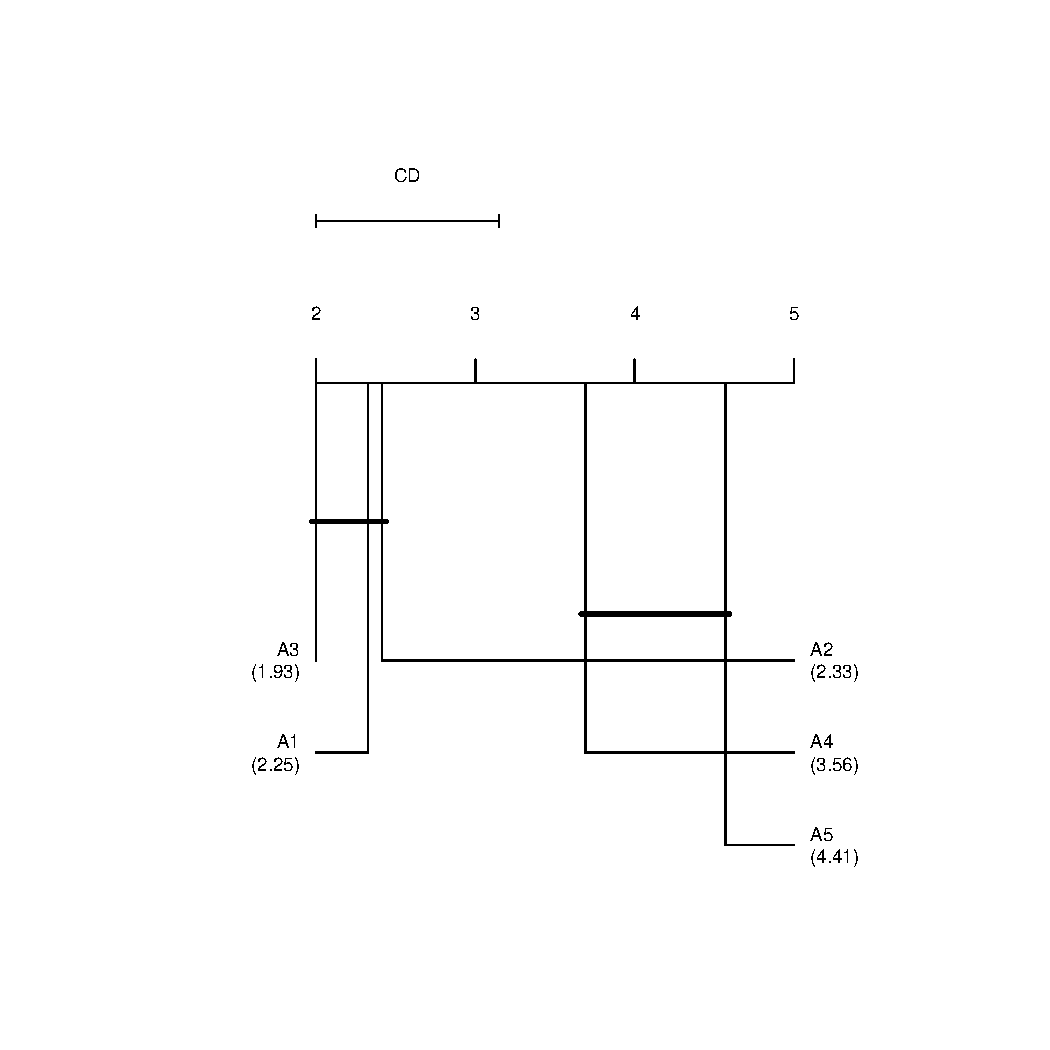
\includegraphics[scale=0.4]{imagens/exemplo-nemenyi.pdf}
    \caption{Exemplo de representação gráfica do teste Nemenyi.}
    \label{fig:ex-nemenyi}
\end{figure}

Observa-se que as abordagens fictícias A3, A1 e A2 formam o grupo de menor valor
de \textit{rank}  médio, e  consequentemente, são  estatisticamente equivalentes
entre si de acordo com o teste de Nemenyi. Portanto, podemos definir como melhor
algoritmo aquele  que apresenta o  maior número de  vitórias, i.e., o  número de
vezes que cada abordagem foi melhor que as demais.

Outro  teste  utilizado  neste  trabalho  foi o  de  Wilcoxon,  aplicado  quando
deseja-se verificar  se existe DES  entre os  resultados de dois  métodos, sendo
mais  poderoso que  o teste  de  Iman-Davenport para  esse cenário.  O teste  de
Wilcoxon computa os  \textit{ranks} das diferenças entre os  resultados dos dois
métodos  ignorando  o  sinal  e posteriormente  compara  os  \textit{ranks}  das
diferenças positivas e negativas.

Para computar  o teste de  Wilcoxon, considere $d_i, i  \in \{1, \dots,  N\}$, a
diferença  entre  os  resultados  das  duas  abordagens  na  i-ésima  instância,
$r_{d_i}$ o \textit{rank} do valor  absoluto da i-ésima diferença (\textit{rank}
médio é  atribuído no caso  de empate). Assuma  $R^+$ a soma  dos \textit{ranks}
para as instâncias nas quais a abordagem fictícia  A foi melhor do que B ($d_i >
0$) e  $R^{-}$ a  soma dos  \textit{ranks} para o  caso oposto  ($d_i <  0$). Os
\textit{ranks} para  $d_i =  0$ são  separados igualmente  entre as  somas, como
mostrado na Equação \eqref{eq:r-wilcoxon}.

\begin{equation}
    R^{+} = \sum_{d_i > 0} r_{d_i} + \frac{1}{2}\sum_{d_i = 0} \quad \quad R^{-} = \sum_{d_i < 0} r_{d_i} + \frac{1}{2}\sum_{d_i = 0} \label{eq:r-wilcoxon}
\end{equation}

Seja T = $\min\{R^+, R^{-}\}$ . Segundo Dem\v{s}ar \cite{demsar:2006}, nos casos
onde $N \leq 25$,  o valor crítico para o teste de  Wilcoxon pode ser consultado
na  maioria  dos   livros  de  estatística,  como  por  exemplo,   o  de  Devore
\cite{devore:2011}. Uma  vez que  tal valor é  calculado, rejeita-se  a hipótese
nula se o valor de $T$ for menor ou  igual ao valor crítico. No caso em que $N >
25$, computa-se a estatística $z$ como apresentado na Equação \eqref{eq:z-stat}.
Segundo Dem\v{s}ar,  considerando um  nível de confiança  de $95\%$,  a hipótese
nula pode ser rejeitada quando $z < -1.96$.

\begin{equation}
    z = \frac{T - \frac{1}{4} N(N + 1)}{\sqrt{\frac{1}{24} N(N+1)(2N + 1)}} \label{eq:z-stat}
\end{equation}

\section{Geração de Instâncias} \label{sec:instance-generation}

Nos  trabalhos presentes  na literatura  que envolvem  o problema  de roteamento
aplicado a redes veiculares,  não há um consenso entre os  autores em relação às
instâncias utilizadas em  experimentos. Cada autor criou  as próprias instâncias
para validação  do algoritmo  ou protocolo proposto,  como pode-se  observar nos
trabalhos  de   \cite{BITAM2013981,  fazio:2013,   tiago:2019}.  A   geração  de
instâncias descrita nesta  seção é fortemente baseada no trabalho  de Ribeiro et
al. \cite{tiago:2019},  que descreve  uma maneira  coerente de  criar instâncias
para  avaliação  de  algoritmos  de roteamento  em  VANET's  utilizando  modelos
baseados  em simulação  de tráfego.  Nessa  simulação é  possível visualizar  os
movimentos dos  veículos que  são gerados,  além de poder  exportar os  dados de
mobilidade, ou  seja, o posicionamento,  velocidade e  direção de um  veículo em
determinado  instante. Os  dados exportados  do modelo  de mobilidade  podem ser
introduzidos em  um simulador  específico para redes  de comunicação,  como NS-2
\cite{Issariyakul:2010}, NS-3 \cite{Riley2010} e OMNet \cite{Varga:2008}.

Para a  simulação de tráfego e  mobilidade veicular tratada neste  trabalho, foi
escolhida a biblioteca  SUMO (\textit{Simulation of Urban MObility}),  que é uma
ferramenta amplamente  utilizada tanto no  meio acadêmico quanto  empresarial. O
SUMO é acoplado a uma ferramenta externa de simulação de redes, neste caso NS-2,
para fornecer dados realistas de comunicação dos veículos. O NS-2 é um simulador
de eventos discretos direcionados à  pesquisa de rede, inicialmente desenvolvido
pela Universidade de Berkeley e  altamente utilizado pela comunidade científica.
O  NS-2 fornece  um  apoio  substancial para  a  simulação  do funcionamento  de
transmissões, roteamento  e protocolos  de redes,  com e  sem fio.  É importante
utilizar o modelo de mobilidade gerado  pelos simuladores de veículos para que o
posicionamento dos nós esteja o mais próximo possível da realidade.

O  primeiro passo  na geração  de instâncias  para o  \gls{pma} é  a criação  de
estradas  e  rodovias.  Neste  trabalho   foram  adotados  como  base  os  mapas
disponíveis no projeto \textit{Open  Street Maps} (OSM) \cite{harklay:2008}, que
é um projeto de  mapeamento colaborativo para criar um mapa  livre e editável do
mundo e está  em desenvolvimento desde 2004.  A Figura \ref{fig:map-open-street}
apresenta  uma   parte  do  mapa  da   cidade  de  Washington  D.   C.,  medindo
aproximadamente 250.000 metros quadrados.

\begin{figure}[!ht]
    \centering
    \fbox{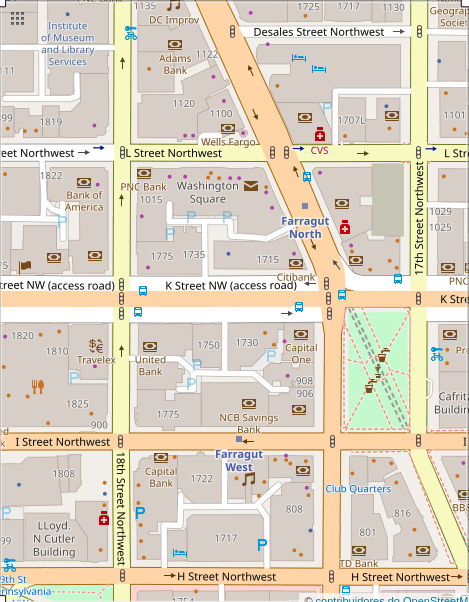
\includegraphics[scale = 0.35]{imagens/map-open-street.png}}
    \caption{Parte do mapa da cidade de Washington no \textit{Open Street Maps}}
    \label{fig:map-open-street}
\end{figure}

O passo seguinte  é tratar e selecionar  as informações desejadas com  o OSM, ou
seja, o  recorte do  mapa que  se deseja  utilizar. Os  dados são  convertidos e
importados para o SUMO gerando assim  o modelo de mobilidade, inserindo veículos
no mapa,  bem como  semáforos e  outros componentes  inerentes ao  tráfego. Após
essas  inserções,  inicia-se  o  processo  de  simulação  do  tráfego  veicular,
exportando  os dados  de  movimentação  dos veículos  para  utilização na  etapa
posterior. A Figura  \ref{fig:map-sumo} apresenta uma parte ampliada  do mapa de
Washington, ressaltando dados de tráfego e veículos.

\begin{figure}[!ht]
    \centering
    \fbox{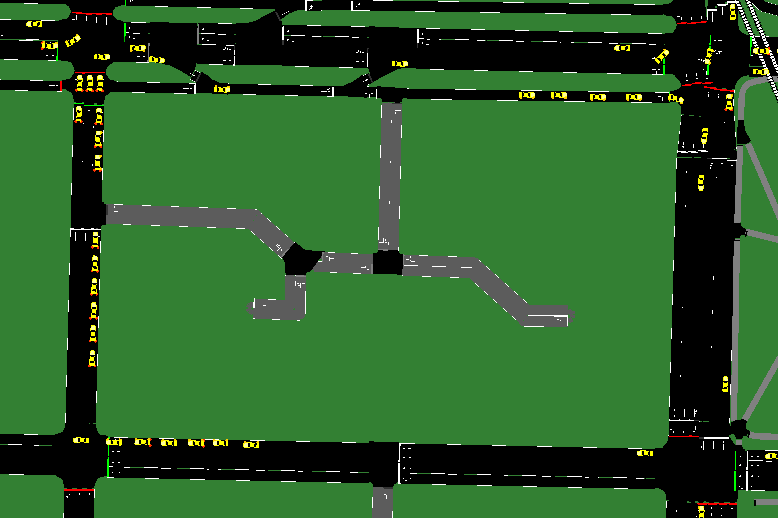
\includegraphics[scale = 0.35]{imagens/map-sumo.png}}
    \caption{Parte do mapa ampliado da cidade de Washington no SUMO}
    \label{fig:map-sumo}
\end{figure}

Após a exportação dos dados vindos do SUMO, será feita a utilização do simulador
de rede  NS-2. O processo  de simulação  de rede é  então iniciado e,  durante o
mesmo, é possível fotografar um momento qualquer e com isso obter a topologia da
rede como um todo,  representando-a como um grafo. O valor  das métricas em cada
\textit{link} é medido com base na troca de mensagem entre os pares de veículos.
Considera-se o  cálculo médio em um  intervalo de 15 segundos.  Assim é possível
ter uma  instância próxima da  realidade, dentro  das limitações do  processo de
simulação.

A Figura \ref{fig:instance}  ilustra o grafo da instância final  gerada a partir
de  um intervalo  de tempo  da  simulação. Os  nós não  seguem o  posicionamento
geográfico real, apenas exibem as conexões existentes naquele intervalo entre os
10 veículos da rede. O nó azul representa a origem, os nós vermelhos representam
os destinos, ambos  decididos aleatoriamente. Os nós pretos são  nós de Steiner,
que  podem  ser   utilizados  ou  não  no  processo  de   construção  da  árvore
\textit{multicast}.

\begin{figure}[!ht]
    \centering
    \fbox{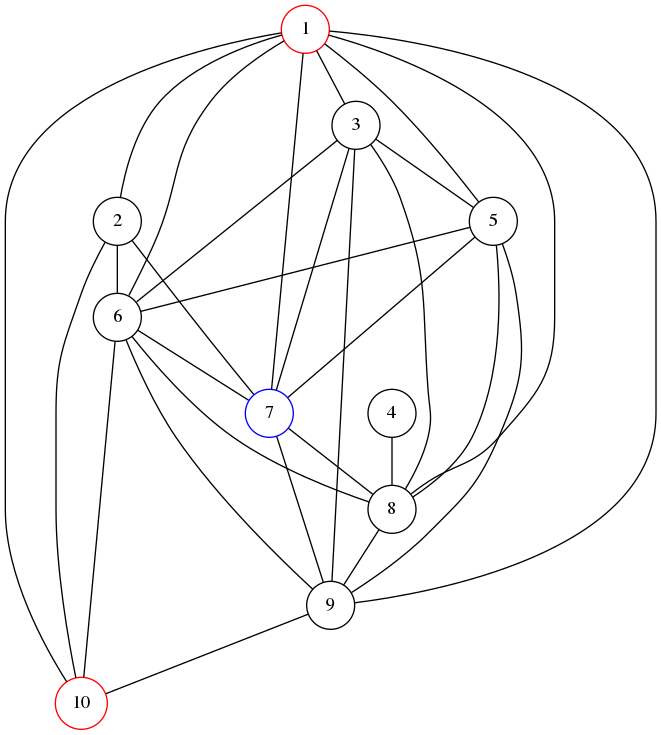
\includegraphics[scale = 0.3]{imagens/instance.png}}
    \caption{Fotografia dos enlaces da rede.}
    \label{fig:instance}
\end{figure}

Outros parâmetros  da instância são os  valores máximos de {\delay}  e {\jitter}
permitidos no  caminho da  raiz até  cada um  dos terminais,  o valor  máximo da
variação de  {\delay} entre o  nó origem  e qualquer par  de destinos e  o valor
mínimo  de largura  de  banda dos  arcos. Foram  gerados  diferentes valores  de
parâmetros  visando  estressar  as  metodologias   na  etapa  de  avaliação  dos
algoritmos.  Para tal,  foram geradas  duas árvores  de caminhos  mínimos do  nó
origem para todos os nós destino. A primeira é calculada utilizando como custo o
{\delay} dos arcos e a segunda o {\jitter}. Essas árvores são referenciadas como
$T^d$ e $T^j$, respectivamente.

Seja $\lambda^{*}$ o maior valor de  {\delay} entre os caminhos da árvore $T^d$.
A partir da árvore  $T^j$, é possível inverter os custos  de {\jitter} dos arcos
pelos  de {\delay}  e assim  obter  $\tilde{\lambda}$, que  é o  maior valor  de
{\delay} nos caminhos  da árvore de {\jitter}, ou seja,  $T^j$. Seguindo o mesmo
procedimentos,   obtém-se   os   valores  $\xi^{*}$   e   $\tilde{\xi}$,   sendo
respectivamente o maior valor de {\jitter} da árvore $T^j$ e da árvore $T^d$.

Para  a  geração   das  instâncias,  os  parâmetros   foram  configurados  como:
$\Delta_{d} = \tilde{\lambda}$  e $\Delta_{j} = \tilde{\xi}$. O  valor do mínimo
de largura  de banda  necessária para o  link foi fixado  em 200,  utilizando um
parâmetro  aplicado  diretamente  ao  simulador  de  rede.  Por  fim,  assumindo
$\lambda^1,  \dots, \lambda^{|D|}$  como  os valores  de  {\delay} dos  caminhos
mínimos para cada terminal na árvore $T^d$, obtém-se o valor de $\Delta_v$ igual
ao desvio  padrão da diferença  absoluta entre todos os  pares de {\delay  s} em
$\lambda^1, \dots, \lambda^{|D|}$.

A  Figura  \ref{fig:flowchart},  retirada  de  \cite{tiago:2019},  apresenta  um
fluxograma simplificado  do processo de  geração das instâncias,  começando pelo
processo de extração do mapa, passando  pela simulação de tráfego usando o SUMO,
juntamente com  a criação do  modelo de mobilidade  e terminando no  processo de
simulação  no NS-2,  onde  a instância  final  é gerada.  O  conjunto de  testes
desenvolvido neste trabalho  é formado por 40 instâncias criadas  a partir de um
trecho real do mapa da cidade de Washington. Para 30 instâncias o número de nós
varia de 10 a 100,  o número de terminais de 4 a 52 e o  número de arcos de 18 a
4416. Para 10 outras instâncias, o número de nós varia de 125 a 350, o número de
terminais de 55 a 170 e o número de arcos de 2448 a 24446.

\begin{figure}[!ht]
    \centering
    \fbox{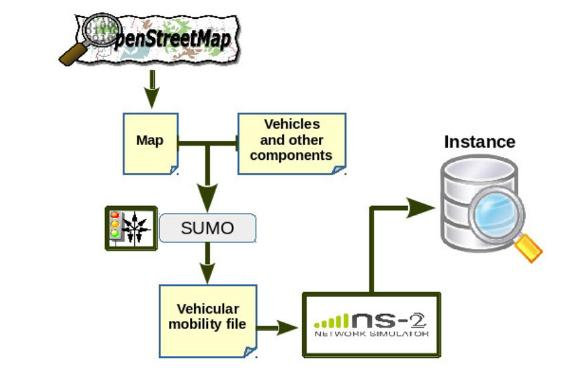
\includegraphics[scale = 0.5]{imagens/flowchart.jpg}}
    \caption{Fluxograma do processo de geração das instâncias.}
    \label{fig:flowchart}
\end{figure}

\begin{comment}
Os  grafos das  instâncias foram  gerados  com base  em 4  recortes de  tamanhos
diferentes do mapa  da cidade de Washington DC, $50^{2}$,  $75^{2}$, $100^{2}$ e
$200^{2}$ na escala de distância da  própria ferramenta. Para cada recorte foram
criadas  10  instâncias,  para  os  3 recortes  menores  o  número  de  veículos
considerados para  o grafo variou  de 10  à 100. Para  o recorte de  $200^{2}$ o
número de veículos foi de 125 a 350. O número de conexões variou de acordo com a
simulação  de  rede  e o  percurso  dos  veículos,  mas  o objetivo  foi  formar
instâncias mais densas  no recorte menor e ir torná-las  mais esparsas de acordo
com o  aumento de  tamanho do trecho  do mapa. O  nós raiz  e o conjunto  de nós
terminais  são selecionado  aleatoriamente, sendo  o número  de terminais  em um
intervalo de $40\%$ a $60\%$ do número de nós. O nome de cada instância é gerado
no  seguinte  padrão  ``washington-tamanho do  recorte-$|V|$-$|D|$''.  A  Tabela
\ref{tab:met-instancias} contém  os dados  de cada  instância, juntamente  com o
número de  conexões, denominado por $E$,  ou seja, não é  considerada direção na
conexão.

\begin{table}[!ht]
\centering
\footnotesize{%
\begin{tabular}{llrlrlr}
\hline
\multicolumn{1}{c}{\textbf{Instância}} & \multicolumn{1}{c}{\textbf{}} & \multicolumn{1}{c}{\textbf{|V|}} & \multicolumn{1}{c}{\textbf{}} & \multicolumn{1}{c}{\textbf{|D|}} & \multicolumn{1}{c}{\textbf{}} & \multicolumn{1}{c}{\textbf{|E|}} \\ \hline
washington-50-10-6 &  & 10 &  & 6 &  & 23 \\
washington-50-20-11 &  & 20 &  & 11 &  & 92 \\
washington-50-30-15 &  & 30 &  & 15 &  & 210 \\
washington-50-40-23 &  & 40 &  & 23 &  & 415 \\
washington-50-50-28 &  & 50 &  & 28 &  & 624 \\
washington-50-60-35 &  & 60 &  & 35 &  & 906 \\
washington-50-70-37 &  & 70 &  & 37 &  & 1258 \\
washington-50-80-39 &  & 80 &  & 39 &  & 1796 \\
washington-50-90-51 &  & 90 &  & 51 &  & 2109 \\
washington-50-100-45 &  & 100 &  & 45 &  & 2208 \\ \hline
washington-75-10-4 &  & 10 &  & 4 &  & 16 \\
washington-75-20-12 &  & 20 &  & 12 &  & 63 \\
washington-75-30-16 &  & 30 &  & 16 &  & 159 \\
washington-75-40-21 &  & 40 &  & 21 &  & 269 \\
washington-75-50-30 &  & 50 &  & 30 &  & 438 \\
washington-75-60-25 &  & 60 &  & 25 &  & 628 \\
washington-75-70-42 &  & 70 &  & 42 &  & 850 \\
washington-75-80-48 &  & 80 &  & 48 &  & 1252 \\
washington-75-90-47 &  & 90 &  & 47 &  & 1517 \\
washington-75-100-52 &  & 100 &  & 52 &  & 1896 \\ \hline
washington-100-10-6 &  & 10 &  & 6 &  & 9 \\
washington-100-20-10 &  & 20 &  & 10 &  & 49 \\
washington-100-30-12 &  & 30 &  & 12 &  & 103 \\
washington-100-40-18 &  & 40 &  & 21 &  & 211 \\
washington-100-50-27 &  & 50 &  & 27 &  & 298 \\
washington-100-60-34 &  & 60 &  & 34 &  & 427 \\
washington-100-70-39 &  & 70 &  & 39 &  & 602 \\
washington-100-80-32 &  & 80 &  & 32 &  & 882 \\
washington-100-90-43 &  & 90 &  & 43 &  & 1151 \\
washington-100-100-43 &  & 100 &  & 43 &  & 1408 \\ \hline
washington-200-125-55 &  & 125 &  & 55 &  & 1224 \\
washington-200-150-61 &  & 150 &  & 61 &  & 2234 \\
washington-200-175-74 &  & 175 &  & 74 &  & 3024 \\
washington-200-200-114 &  & 200 &  & 114 &  & 3645 \\
washington-200-225-135 &  & 225 &  & 135 &  & 4464 \\
washington-200-250-109 &  & 250 &  & 109 &  & 6403 \\
washington-200-275-146 &  & 275 &  & 146 &  & 7195 \\
washington-200-300-136 &  & 300 &  & 136 &  & 8709 \\
washington-200-325-170 &  & 325 &  & 170 &  & 9260 \\
washington-200-350-150 &  & 350 &  & 150 &  & 12218 \\ \hline
\end{tabular}%
}
\caption{Sumário das instâncias}
\label{tab:met-instancias}
\end{table}
\end{comment}